\documentclass[11pt,letterpaper,final]{report}
\usepackage[utf8]{inputenc}
\usepackage[francais]{babel}
\usepackage[T1]{fontenc}
\usepackage{amsmath}
\usepackage{amsfonts}
\usepackage{amssymb}
\usepackage{graphicx}
\usepackage{lmodern}
\usepackage[stable]{footmisc}
\usepackage{pdfpages}
\usepackage[left=2.54cm,right=2.54cm,top=2.54cm,bottom=2.54cm]{geometry}
\begin{document}
\chapter{Validation croisée entre les différentes plateformes de simulations}
Ce chapitre présente une comparaison des simulateurs selon les paramètres des simulation critiques: courant dans les électroaimants, tension aux bornes des électroaimants, courant à l'entrée de l'AFE, tension du bus CC, courants et tensions dans les IGBT. Les sous-modèles se séparent en plusieurs catégories, soit les simulations représentant l'AFE, ceux représentant le convertisseur CC-CC et ceux représentant un montage avec un AFE et un convertisseur CC-CC. Il est à noté que le temps de simulation qui est employé pour fins d'analyse est de 1$\mu$s. 

\section{Comparaison entre PSIM et SPS}
Cette section décrit des comparaisons faites sur le fonctionnement des éléments de bases fondamentaux pour le projet, dans les simulateurs PSIM et SPS.
\subsection{Algorithmes de simulation sur PSIM et SPS}
PSIM et SPS utilisent des méthodes de résolution différentes. SPS est un outil de simulation puissant et générique. Il établit un système d'équations d'états à partir du modèle de simulation, ces équations permettant de déterminer la solution du circuit. Les éléments non-linéaires sont modélisés comme des sources de courants. Les interrupteurs sont modélisés par une faible résistance en conduction et une forte résistance en blocage. Afin d'obtenir des modèles discrets, SPS discrétise les équations d'états continues en utilisant la méthode de Tustin  \footnote{http://www.mathworks.com/products/simpower/description4.html, 17 avril 2014}, la figure \ref{fig_solving_SPS} présente un résumé schématique de l'implémentation. Afin d'augmenter la vitesse de simulation de l'électronique de puissance, SPS utilise un algorithme dans lequel les commutations sont idéales. Il existe deux méthodes de détection des passages par zéro dans SPS , soit la méthode Tustin  (équivalente à une méthode trapézoïdale) et la méthode Backward Euler. La méthode trapézoïdale offre une meilleur précision pour un temps de calcul fixe, mais peut parfois présenter des oscillations numériques. La méthode Backward Euler est moins précise pour un pas de simulation donné, mais permet d'éviter les oscillations numériques. PSIM implémente les modèles au moyen d'une matrice d'admittance nodale\footnote{http://powersimtech.com/support/frequently-asked-questions/, 17 avril 2014}. Les interrupteurs sont idéaux et représentés par une résistance faible en conduction et par une résistance élevée en blocage. La méthode de simulation de PSIM est moins adaptée à l'étude des transitoires pour l'électronique. Elle est cependant plus rapide et permet des études de plus haut niveau. La méthode de détection des passages par zéro de PSIM est une méthode trapézoïdale. 

\begin{figure}
\centering
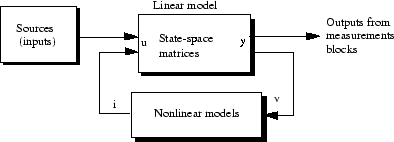
\includegraphics[scale=0.7]{Fig/Comp/improving_performance5.png}
\caption{Méthode de solution des systèmes implantée dans SPS}
\label{fig_solving_SPS}
\end{figure}

\subsection{Comparaison des modèles d'IGBT}

\begin{figure}[htb]
\centering
\includegraphics[scale=0.5]{Fig/Comp/IGBT.jpg}
\caption{Commutation d'un IGBT à un pas de calcul de 5$\mu$s}.
\label{IG}
\end{figure}

Les IGBT sont les interrupteurs utilisés dans chacun des sous-modèles simulés du projet. On remarque sur la figure \ref{IG} que le  courant traversant l'IGBT est identique dans le cas d'un IGBT sur une charge résistive de 50k$\Omega$. Le pas de calcul employé sur les deux plateformes est de 5$\mu$s. L'indice de modulation des IGBT est de 0.5 et la fréquence de commutation de kKHz. Le montage est alimenté par une tension continue de 1kV et possède une résistance interne de 0.01$\Omega$. 

Sur SPS, l'IGBT possède un snubber RC intégré, tandis que sur PSIM il faut l'incorporer manuellement. Pour les deux simulations, le snubber employé est une résistance de 100k$\Omega$.
 
\subsection{Contrôleur proportionnel-intégrateur (PI)}
L'implantation des blocs PI est différente entre SPS et PSIM. Sur SPS, il est possible d'obtenir une forme idéale ainsi qu'une forme parallèle, tandis que sur PSIM, les blocs par défaut ne comportent que la forme idéale. La forme parallèle doit être implantée manuellement. On remarque sur la figure \ref{PI} que les résultats sont identiques entre une implantation manuelle sur PSIM et le bloc par défaut de SPS. La valeur du gain intégrateur du PI est de 50 et celle du gain proportionnel de 0.071. 

\begin{figure}[htb]
\centering
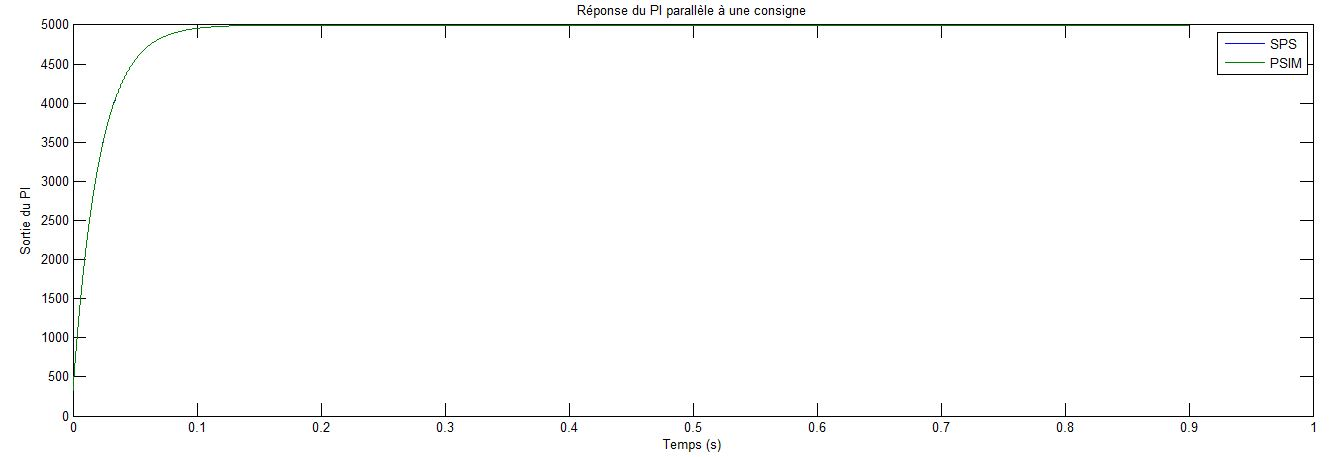
\includegraphics[scale=0.5]{Fig/Comp/PI.jpg}
\caption{Réponse d'un contrôleur PI suite à une consigne d'erreur}.
\label{PI}
\end{figure}

\clearpage
\section{Convertisseur CC-CC 4 quadrants à 4 interrupteurs IGBT}
\subsection{Description du sous-système}
Le hacheur 4 quadrants, à proprement parlé, est constitué de 4 interrupteurs IGBT commandés au moyen d'une régulation MLI. La figure \ref{hach} présente le circuit électrique associé à un tel convertisseur. Ce type de montage est un montage de base utilisé afin de valider le concept de fonctionnement d'un convertisseur CC-CC et d'établir la méthodologie de comparaison des simulations. Le tableau \ref{p_hash} présente les paramètres utilisés pour le hacheur 4 quadrants.

\begin{figure}[htb]
\centering
<<<<<<< HEAD
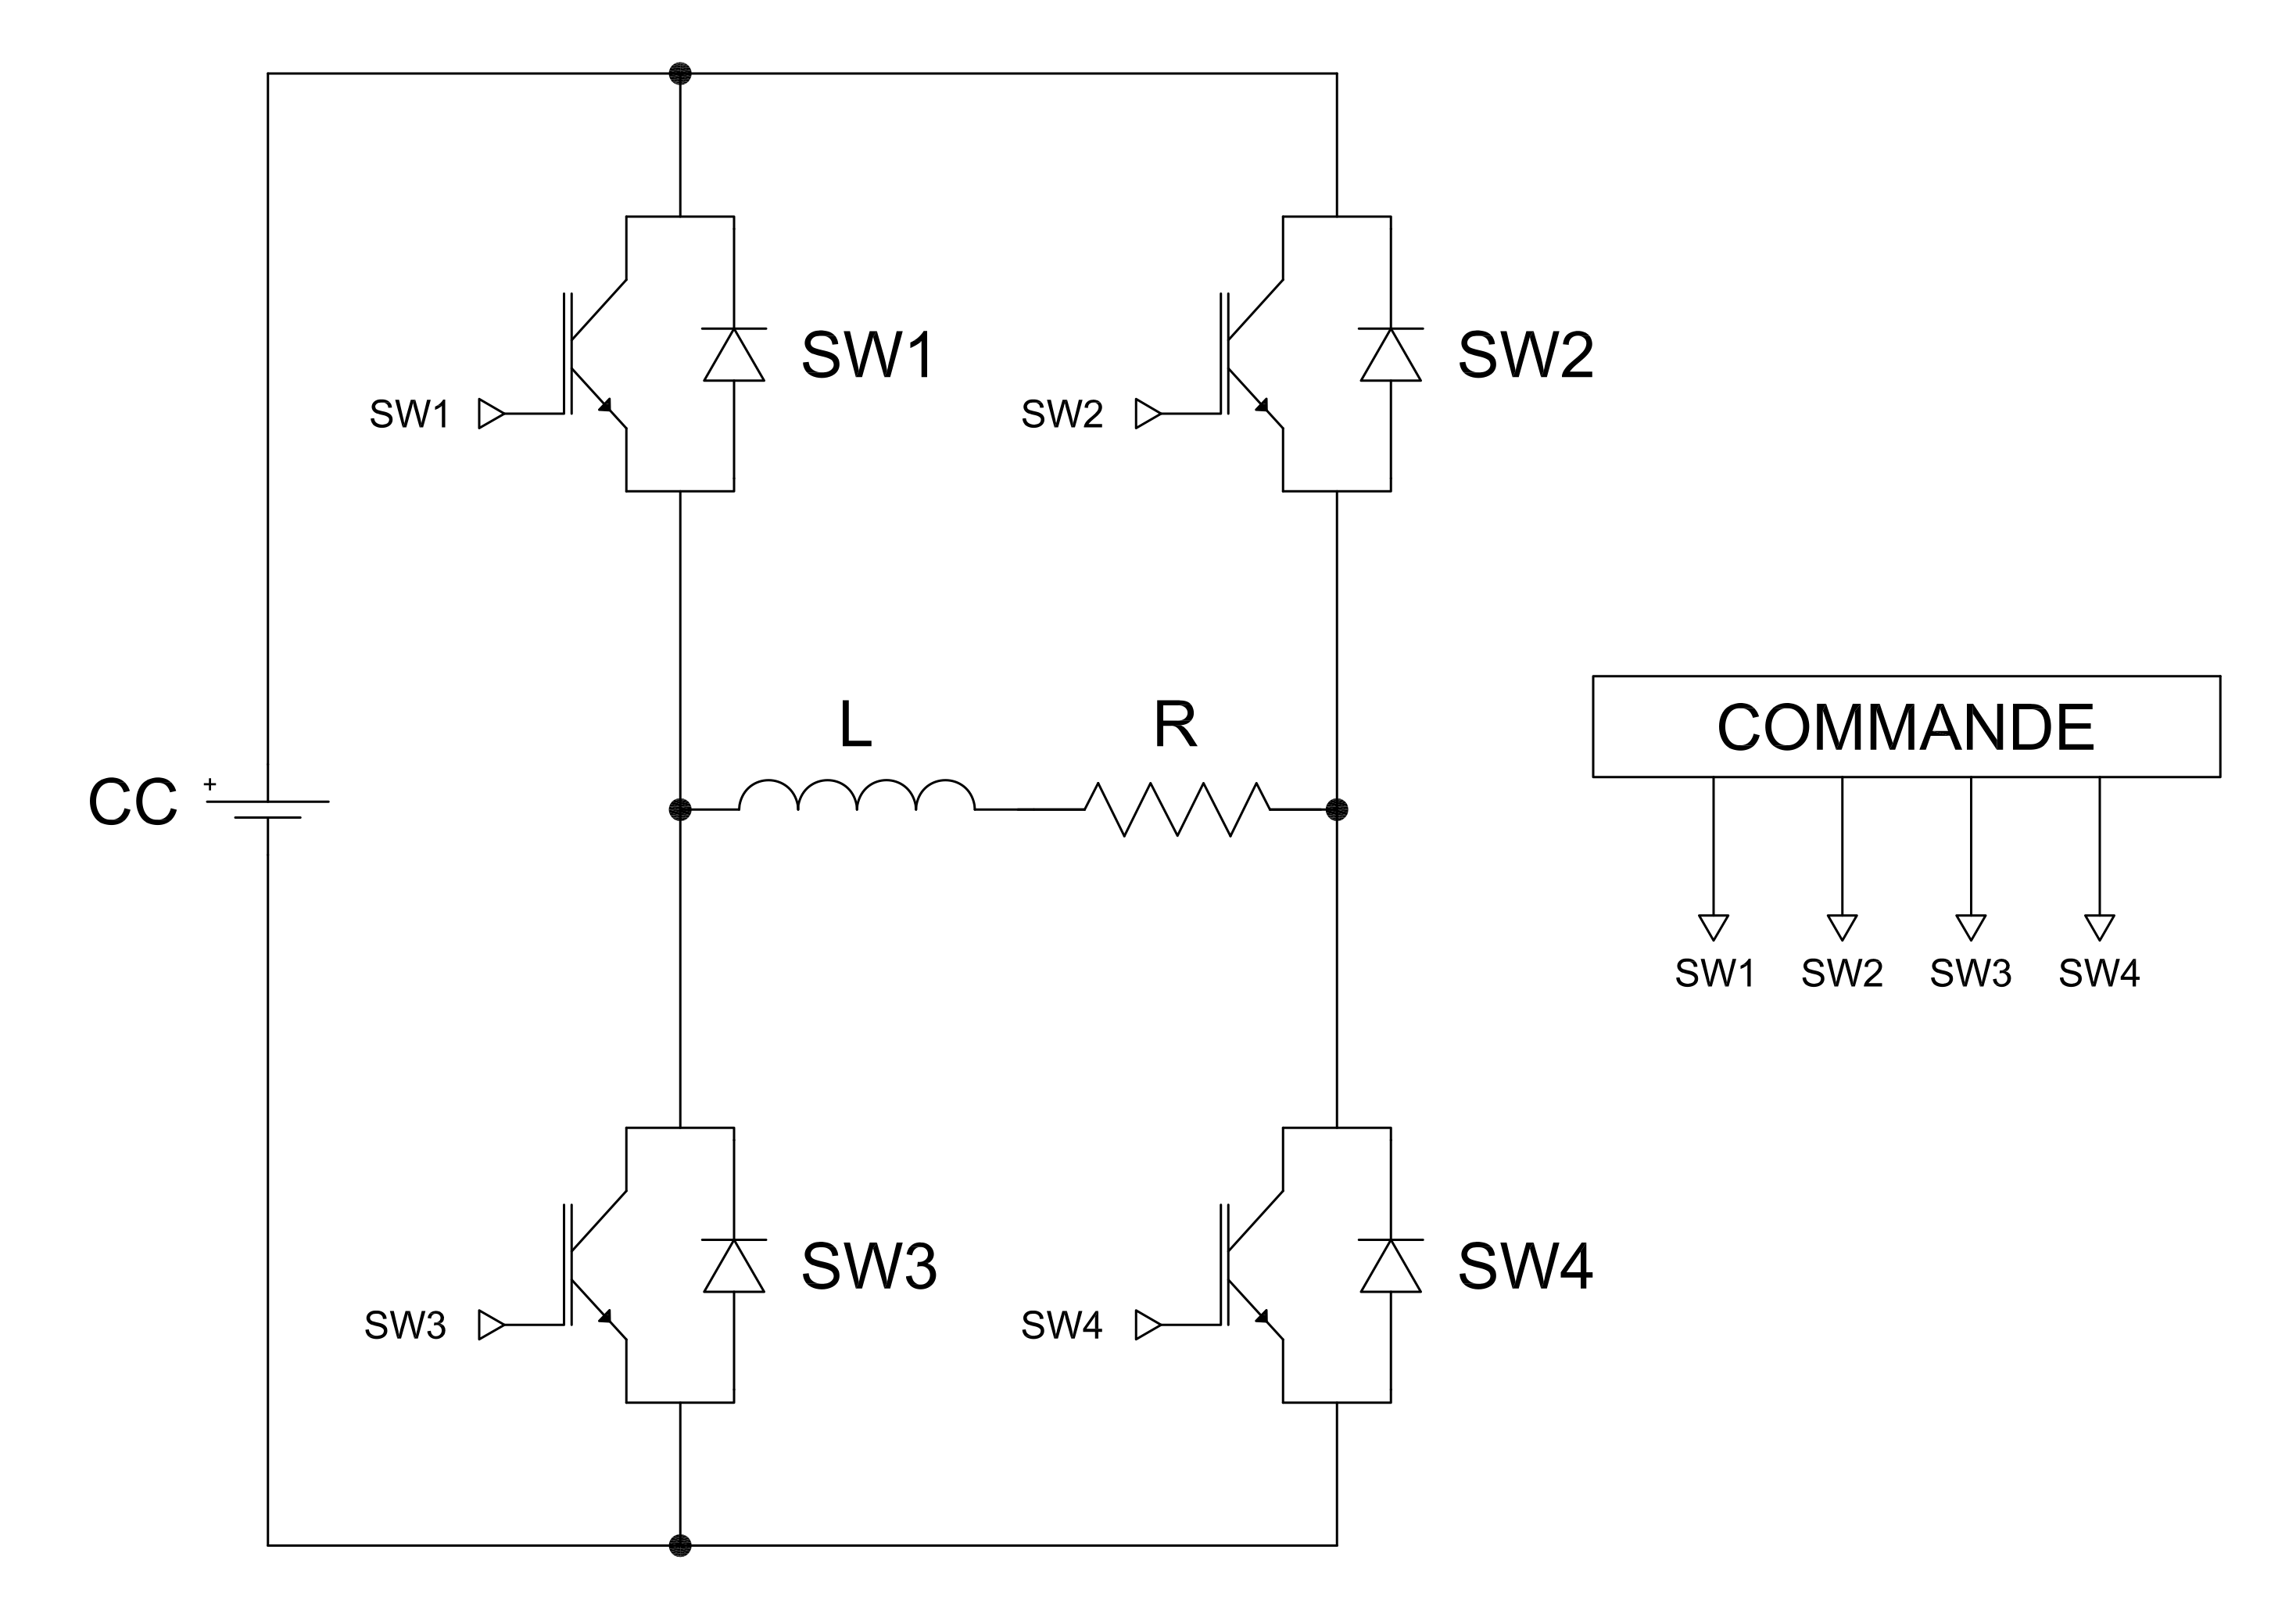
\includegraphics[scale=0.5]{Fig/H4Q.png}
\caption{Circuit électrique du convertisseur CC-CC 4 quadrants à 4 interrupteurs IGBT}.
=======
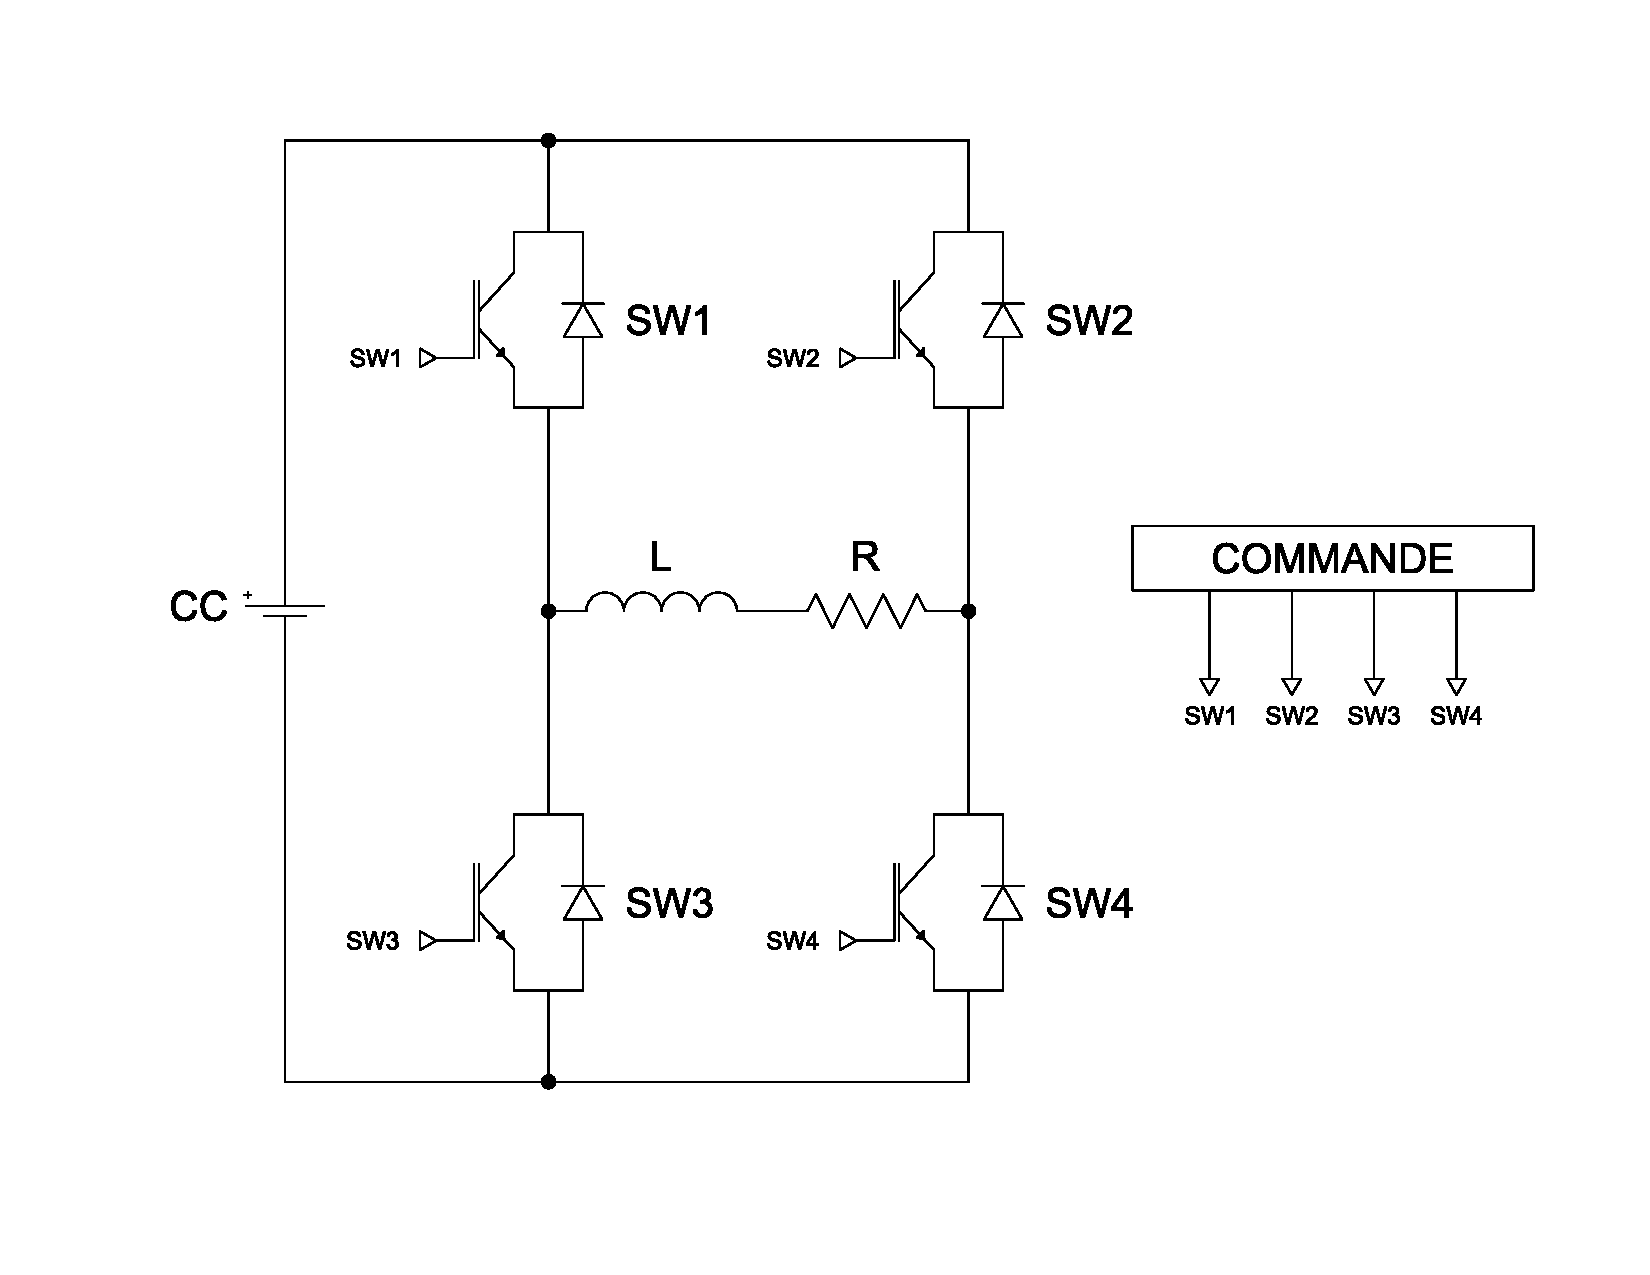
\includegraphics[scale=0.5]{Fig/Hacheur4Quadrants/H4Q.pdf}
\caption{Pont en H à 4 interrupteurs}.
>>>>>>> FETCH_HEAD
\label{hach}
\end{figure}

\begin{table}[htb]
\centering
\begin{tabular}{|l|c|} 
  \hline
  \textbf{Paramètre} & \textbf{Valeur}  \\
  \hline\hline
  Tension CC & 5000 V\\ \hline
  Fréquence de modulation & 1000 Hz\\ \hline
  Rapport cyclique maximal & 0.95 \\ \hline \hline
  \multicolumn{2}{|c|}{\textbf{IGBT}}\\ \hline
  Résistance interne & 0.001 $\Omega$\\
  Résistance du snubber & 100k $\Omega$\\ \hline \hline
   \multicolumn{2}{|c|}{\textbf{PI}}\\ \hline
  Gain proportionnel & 0.071 \\
  Gain intégrateur & 50 \\ \hline \hline
  \multicolumn{2}{|c|}{\textbf{Charge}}\\ \hline
  Résistance & 0.28 $\Omega$\\
  Inductance & 0.1 H\\
  \hline
\end{tabular}
\caption{Paramètres de simulation pour le convertisseur CC-CC à 4 interrupteurs}
\label{p_hash}
\end{table}

\subsubsection{Vérification pour un pas de calcul de 1$\mu$s}
Cette section présente les résultats de simulations du convertisseur CC-CC 4 quadrants, formé avec 4 interrupteurs IGBT, pour un pas de calcul de 1$\mu$s. 


\begin{figure}[htb]
\centering
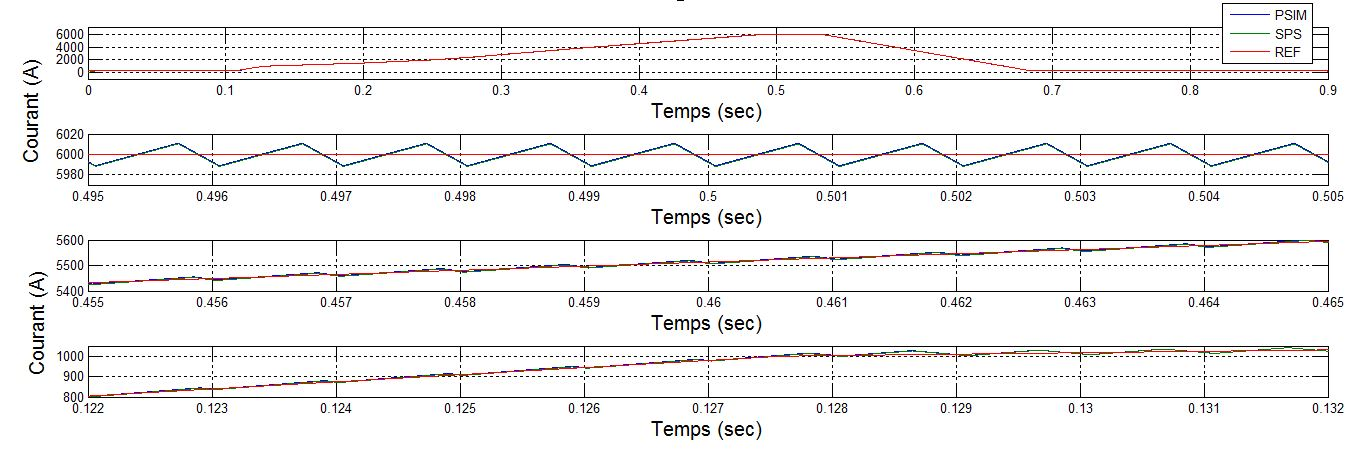
\includegraphics[scale=0.5]{Fig/Hacheur4Quadrants/HacheurCourantCharge1u.jpg}
\caption{Courant traversant la charge sur PSIM et SPS pour un pas de calcul de 1$\mu$s, pour le hacheur 4 quadrants}
\label{hc_cou_ch_1}
\end{figure}


\begin{figure}[htb]
\centering
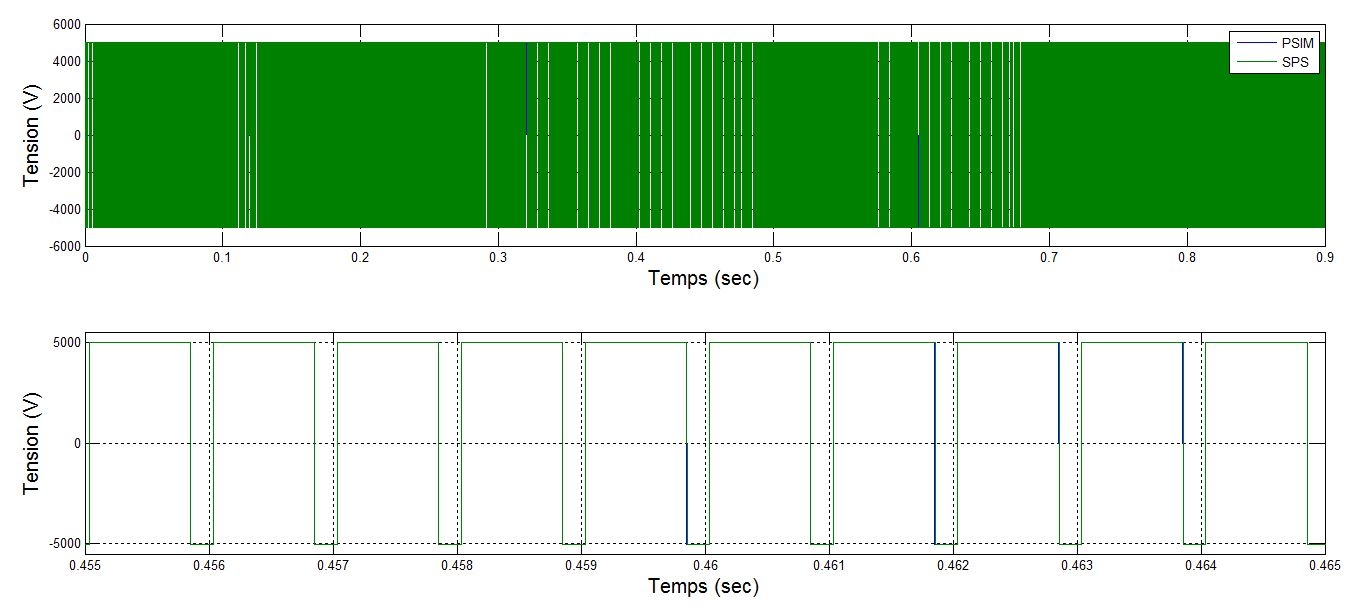
\includegraphics[scale=0.5]{Fig/Hacheur4Quadrants/HacheurTensionCharge1u.jpg}
\caption{Tension aux bornes de la charge sur PSIM et SPS pour un pas de calcul de 1$\mu$s, pour le hacheur 4 quadrants}
\label{hc_ten_ch_1}
\end{figure}


\begin{figure}[htb]
\centering
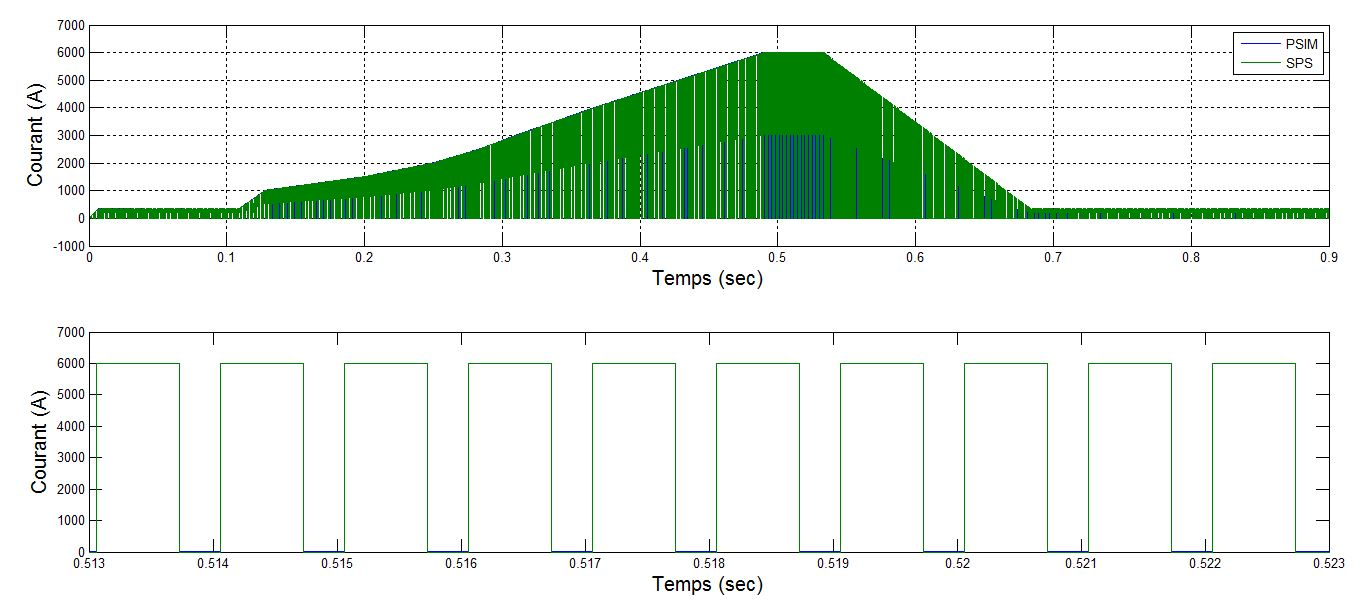
\includegraphics[scale=0.5]{Fig/Hacheur4Quadrants/HacheurCourantIGBT1u.jpg}
\caption{Courant traversant un IGBT sur PSIM et SPS pour un pas de calcul de 1$\mu$s, pour le hacheur 4 quadrants}
\label{hc_IG_cou_1}
\end{figure}

\begin{figure}[htb]
\centering
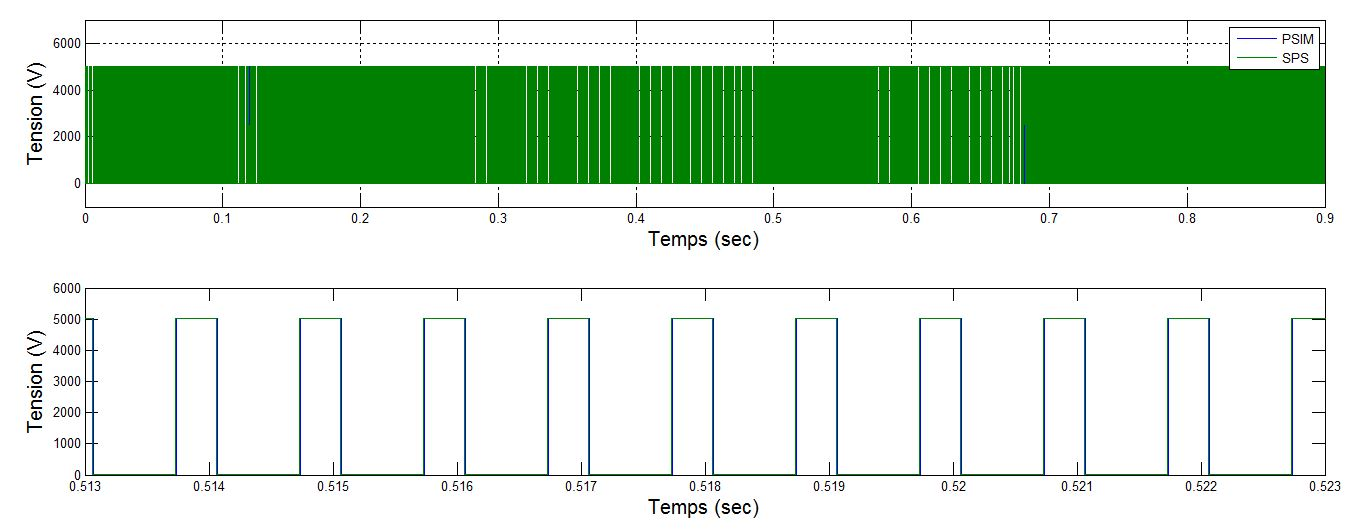
\includegraphics[scale=0.5]{Fig/Hacheur4Quadrants/HacheurTensionIGBT1u.jpg}
\caption{Tension aux bornes d'un IGBT sur PSIM et SPS pour un pas de calcul de 1$\mu$s, pour le hacheur 4 quadrants}
\label{hc_IG_ten_1}
\end{figure}


\clearpage
\section{Convertisseur CC-CC 4 quadrants formé de 2 convertisseurs 3 niveaux NPC}
Le montage implanté au CERN est un convertisseur CC-CC formé de 2 onduleurs triphasés 3 niveaux NPC. La cellule supérieure est dénotée par DCP et la cellule inférieure par DCN. L'assemblage des onduleurs est tel qu'il permet le fonctionnement dans les 4 quadrants. Cette version reproduit le fonctionnement du hacheur 4 quadrants de base avec un plus grand degré de liberté. Il est composé au total de 24 interrupteurs IGBT/DIODE commandé par MLI ainsi que de 12 diodes de point milieu. La figure \ref{circuit_DCP_DCN} présente le circuit électrique du convertisseur. Le tableau \ref{p_DCP} présente les données utilisées pour ce sous-système.


\begin{figure}[htb]
\centering
<<<<<<< HEAD
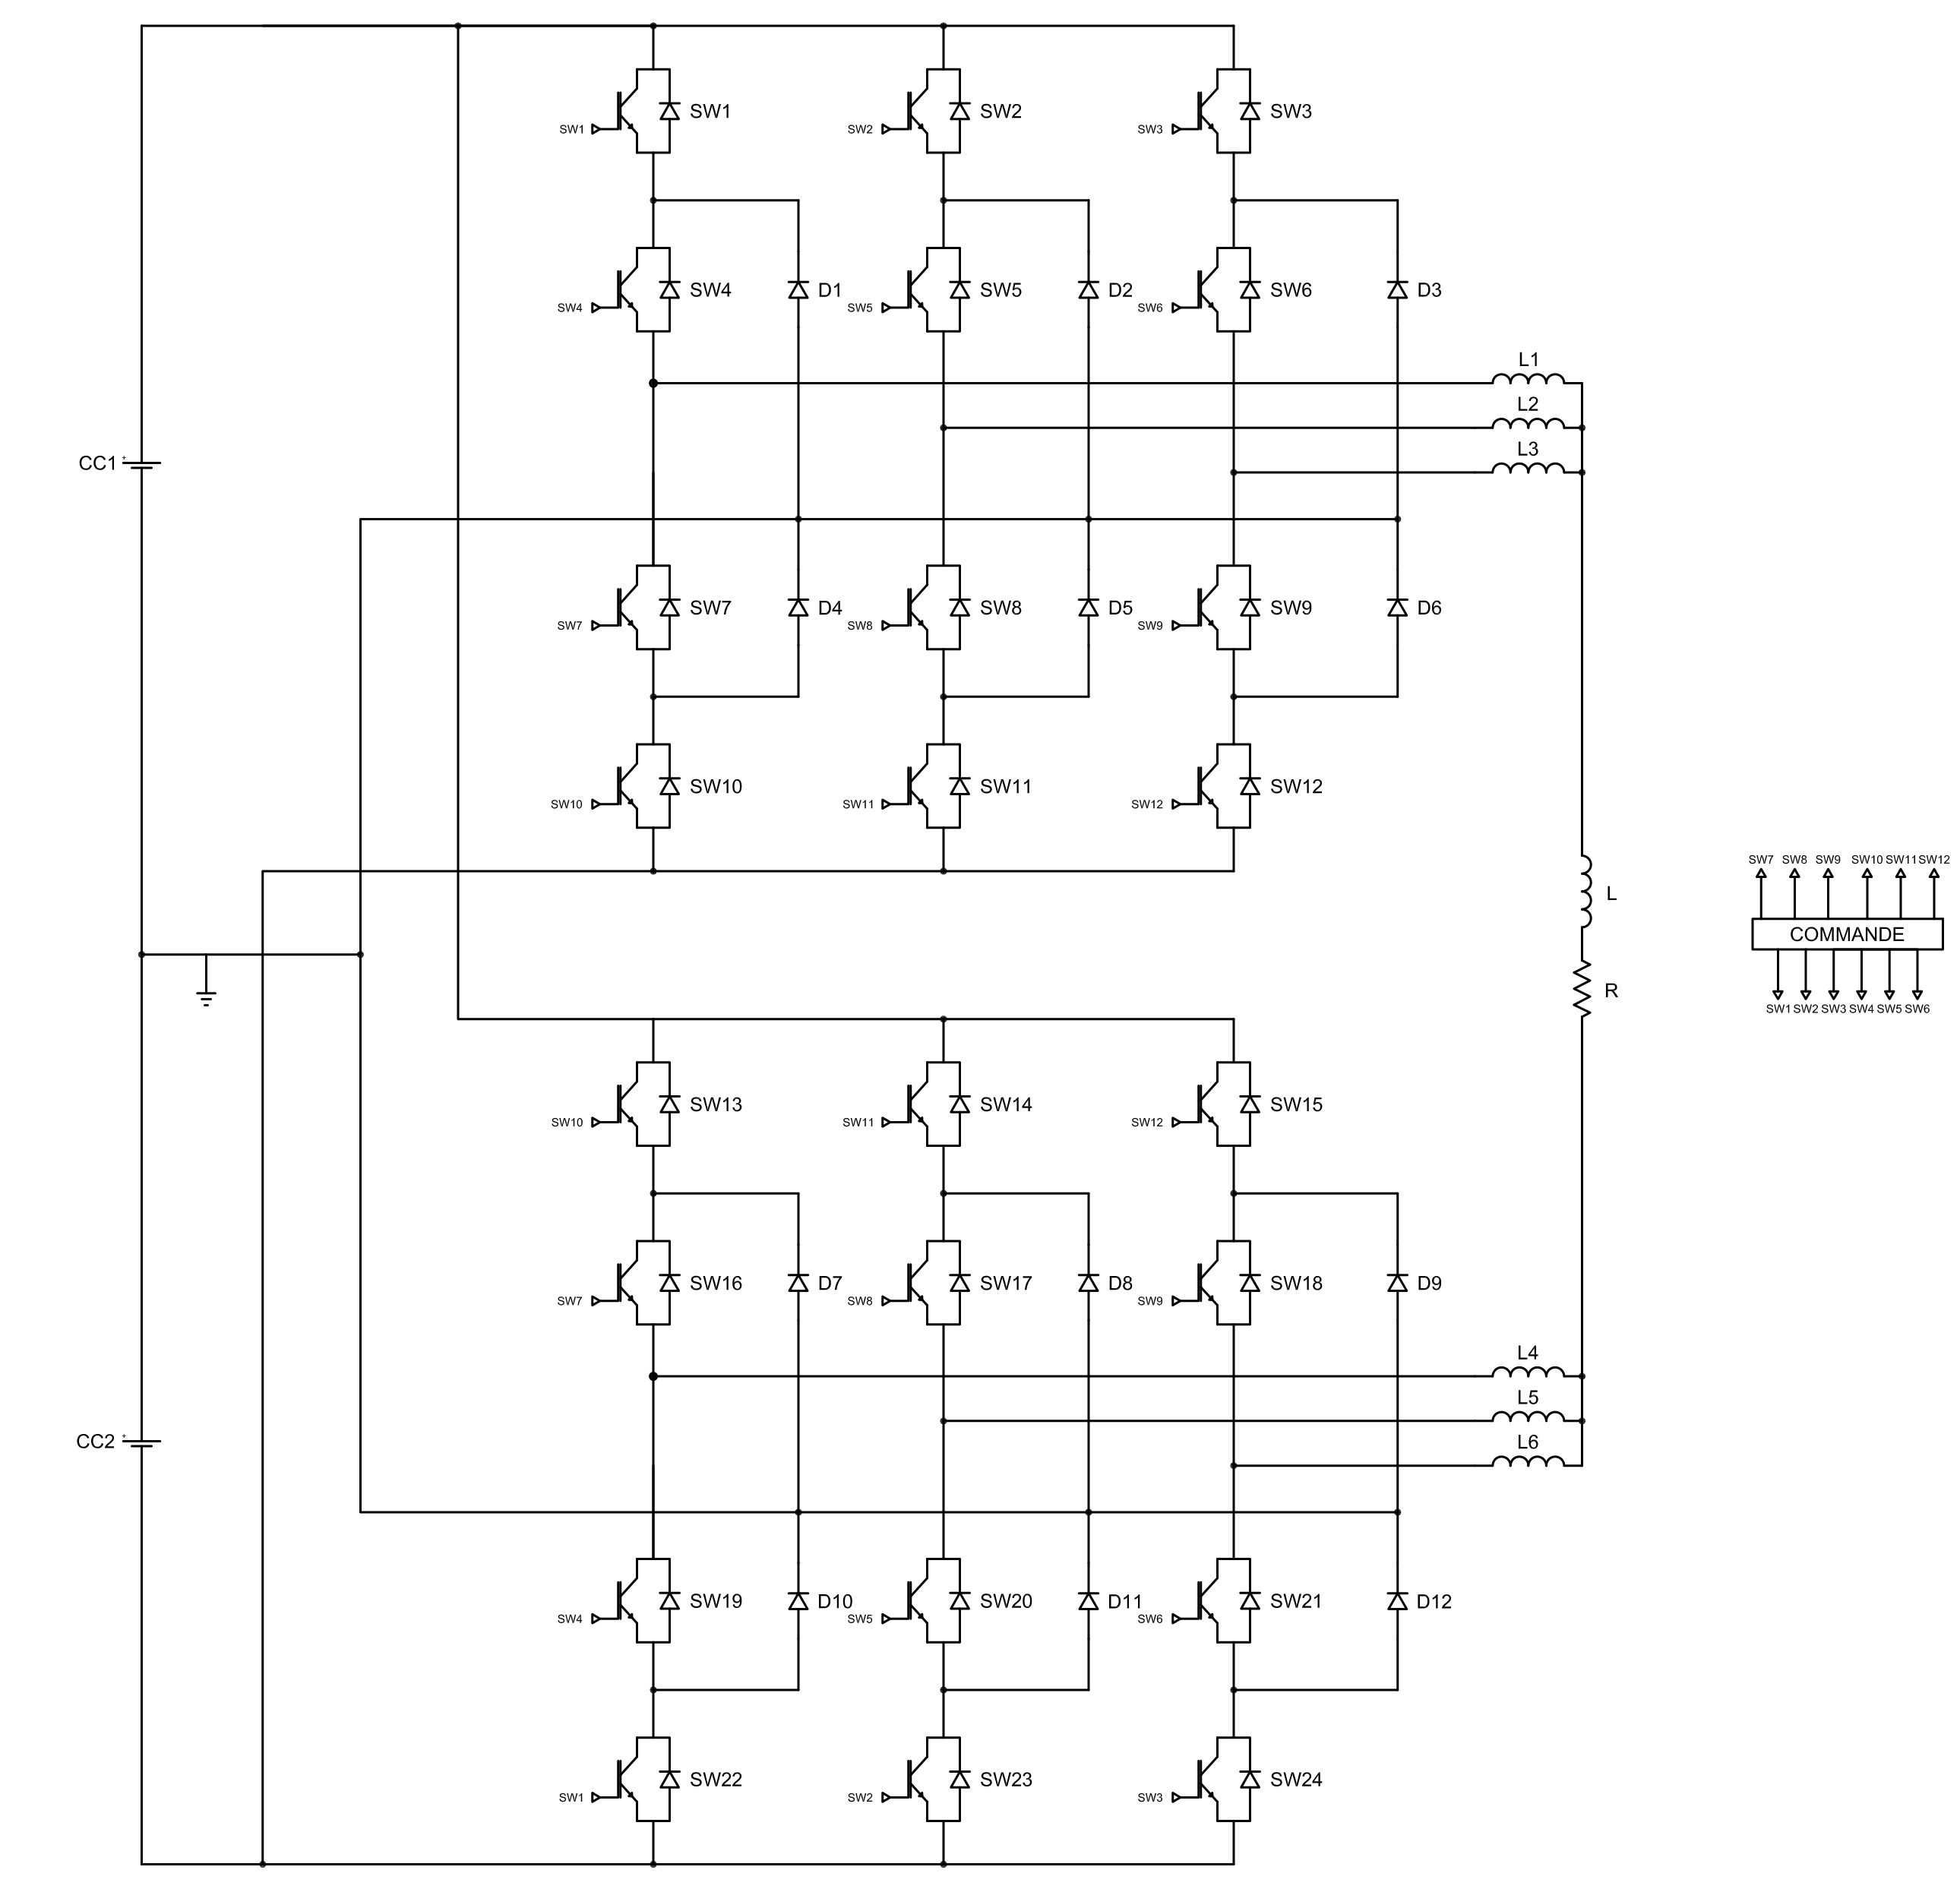
\includegraphics[scale=0.75]{Fig/DCP_DCN.png}
\caption{Circuit électrique du convertisseur CC-CC 4 quadrants formé de 2 convertisseurs 3 niveaux NPC}
\label{circuit_DCP_DCN}
=======
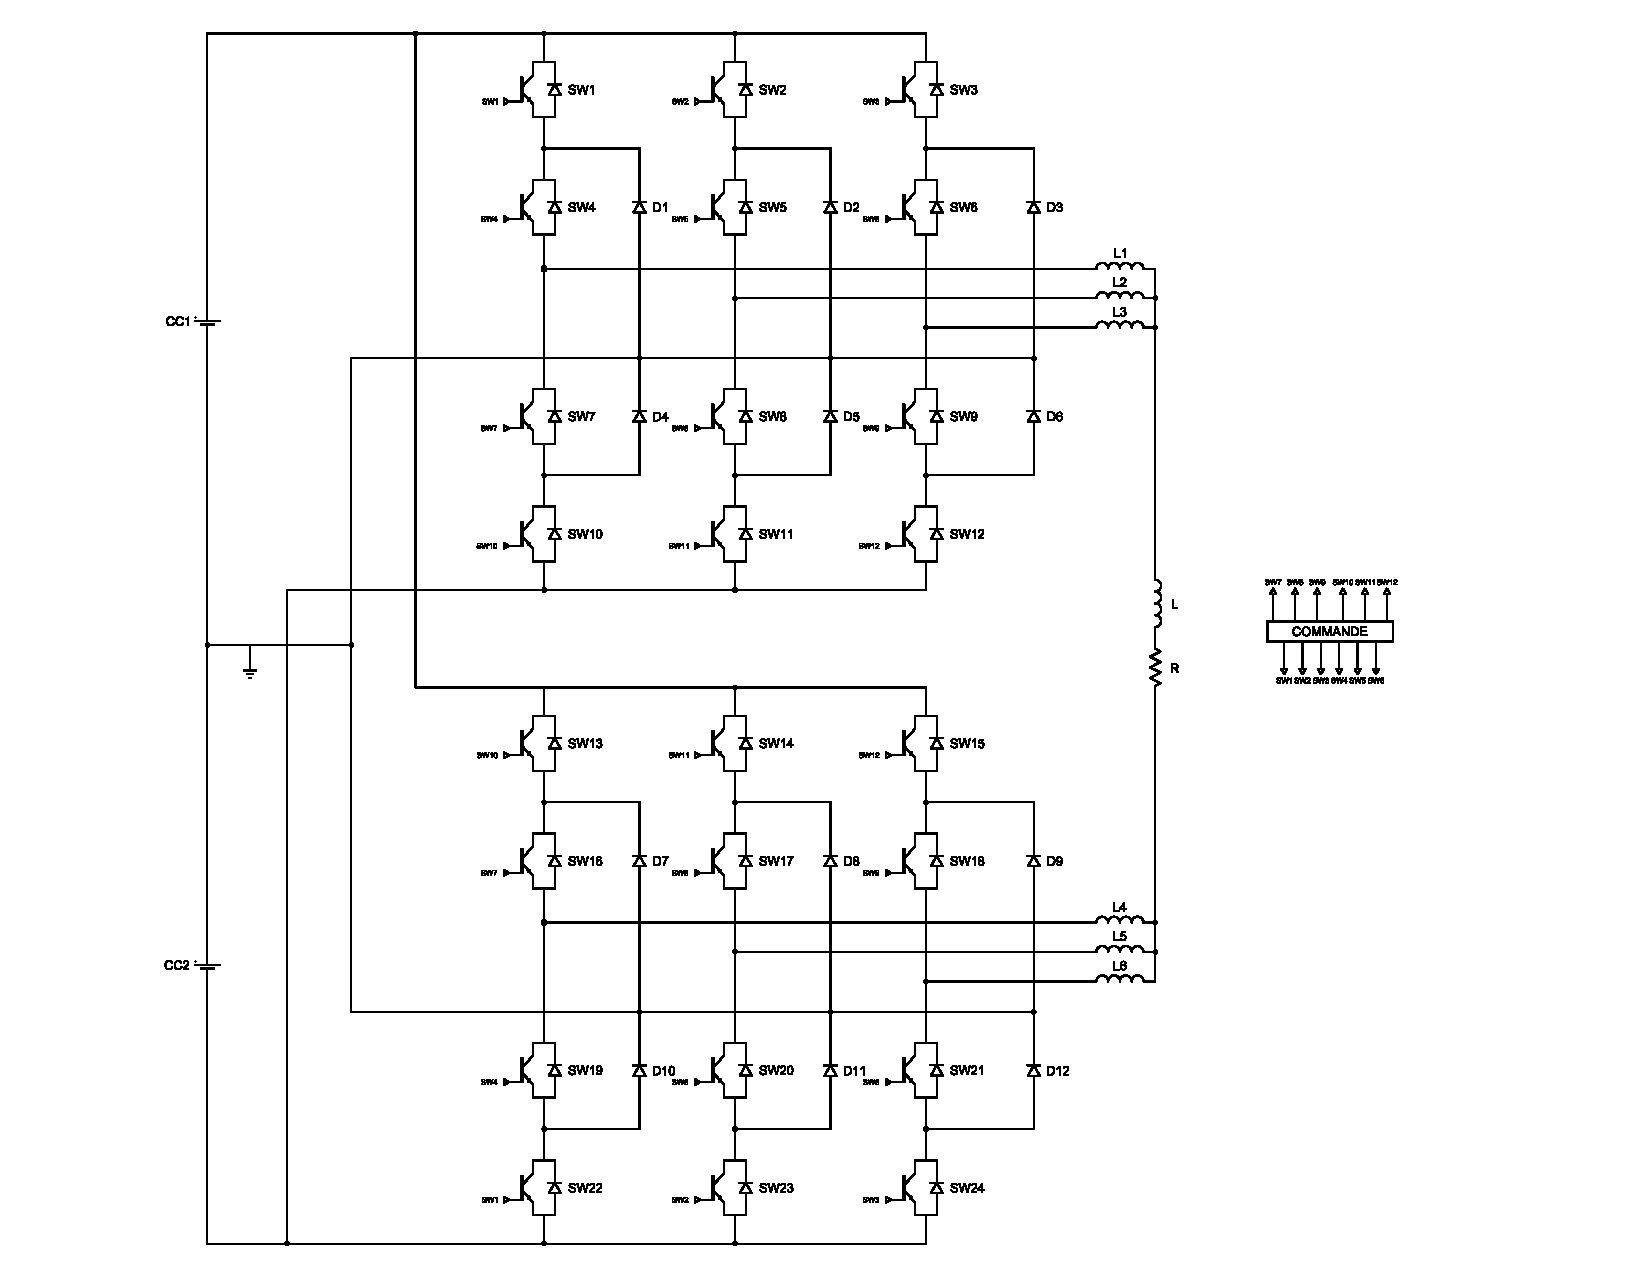
\includegraphics[scale=0.7]{Fig/DCPDCN/DCP_DCN.pdf}
\caption{Schéma bloc du DCP/DCN avec une commande MLI à la charge}
\label{DC_DP}
>>>>>>> FETCH_HEAD
\end{figure}


\begin{table}[htb]
\centering
\begin{tabular}{|l|c|} 
  \hline
  \textbf{Paramètre} & \textbf{Valeur}  \\
  \hline\hline
  Tension CC & 5000 V\\ \hline
  Fréquence de modulation & 1000 Hz\\ \hline
  Rapport cyclique maximal & 1 \\ \hline
  Inductance de couplage & 10e-6 H \\ \hline \hline
  \multicolumn{2}{|c|}{\textbf{IGBT}}\\ \hline
  Résistance interne & 0.001 $\Omega$\\
  Résistance du snubber  & 100k $\Omega$\\ \hline \hline
   \multicolumn{2}{|c|}{\textbf{PI}}\\ \hline
  Gain proportionnel & 1.5611 \\
  Gain intégrateur & 24.6 \\ \hline \hline
  \multicolumn{2}{|c|}{\textbf{Charge}}\\ \hline
  Résistance & 0.28 $\Omega$\\
  Inductance & 0.1 H \\
  \hline
\end{tabular}
\caption{Paramètres de simulation pour le DCP/DCN}
\label{p_DCP}
\end{table}
\clearpage


\subsection{Vérification à un pas de calcul de 1us}
Cette section présente les résultats de simulation obtenus sur PSIM et SPS pour le convertisseur CC-CC 4 quadrants formé de 2 cellules NPC 3 niveaux, pour un pas de calcul discret de 1$\mu$s.



\begin{figure}[htb]
\centering
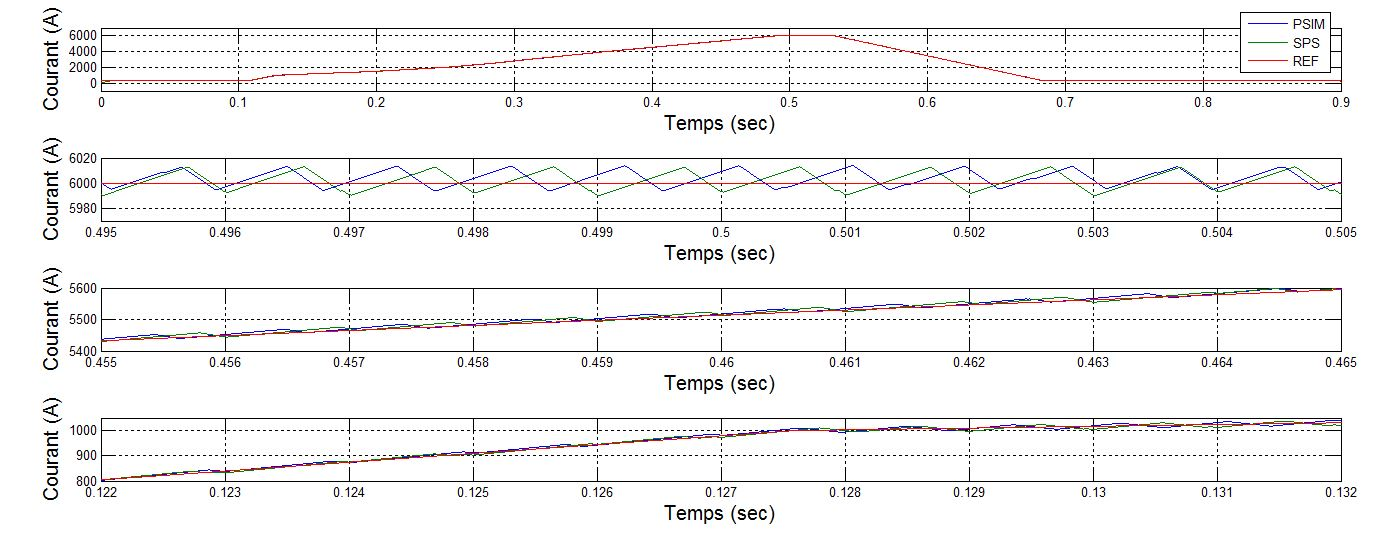
\includegraphics[scale=0.5]{Fig/DCPDCN/DCPCourantCharge1u.jpg}
\caption{Courant traversant la charge sur PSIM et SPS pour un pas de calcul de 1$\mu$s pour le DCP/DCN}
\label{DC_ch_cou_1}
\end{figure}



\begin{figure}[htb]
\centering
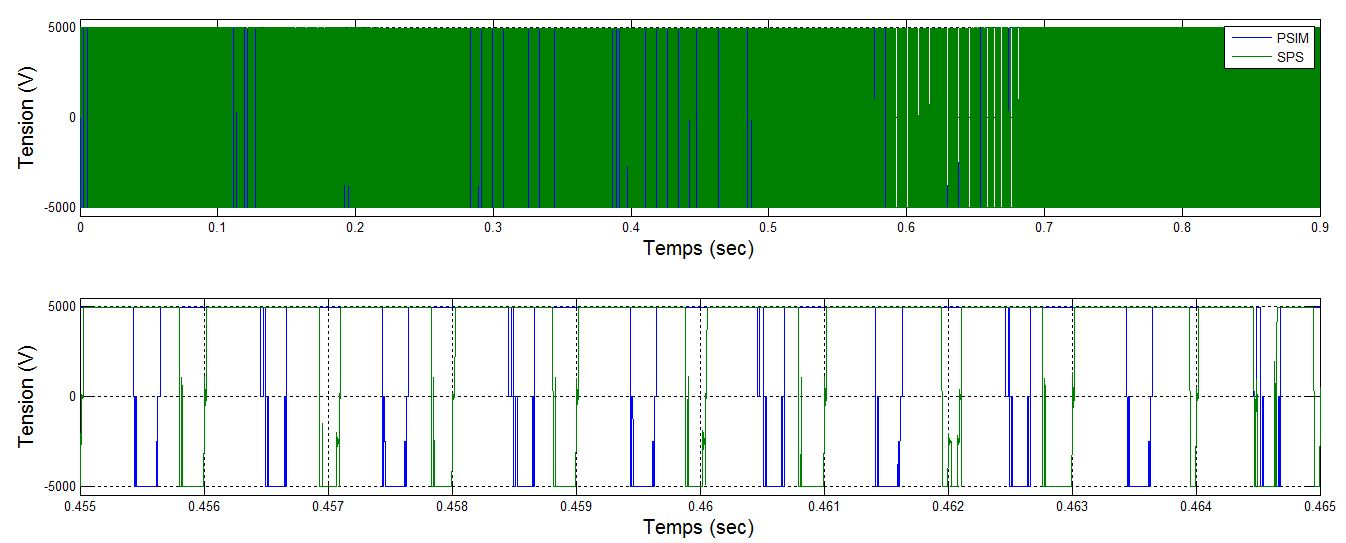
\includegraphics[scale=0.5]{Fig/DCPDCN/DCPTensionCharge1u.jpg}
\caption{Tension aux bornes de la charge sur PSIM et SPS pour un pas de calcul de 1$\mu$s pour le DCP/DCN}
\label{DC_ch_ten_1}
\end{figure}


\begin{figure}[htb]
\centering
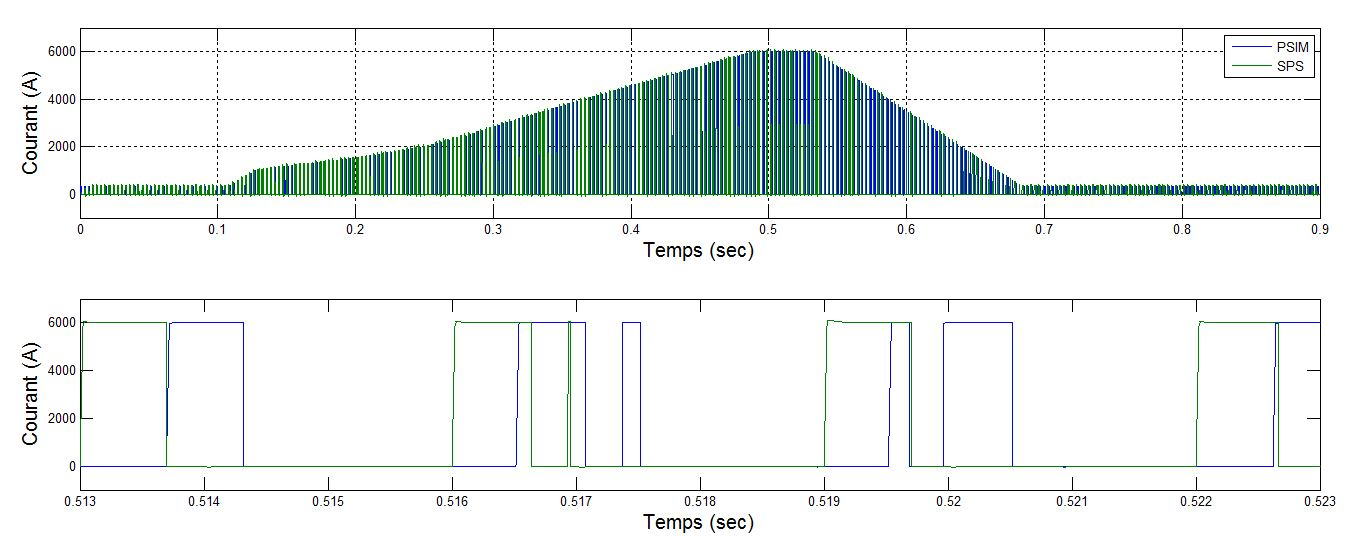
\includegraphics[scale=0.5]{Fig/DCPDCN/DCPCourantIGBT1u.jpg}
\caption{Courant traversant un IGBT sur PSIM et SPS pour un pas de calcul de 1$\mu$s pour le DCP/DCN}
\label{DC_IG_cou_1}
\end{figure}


\begin{figure}[htb]
\centering
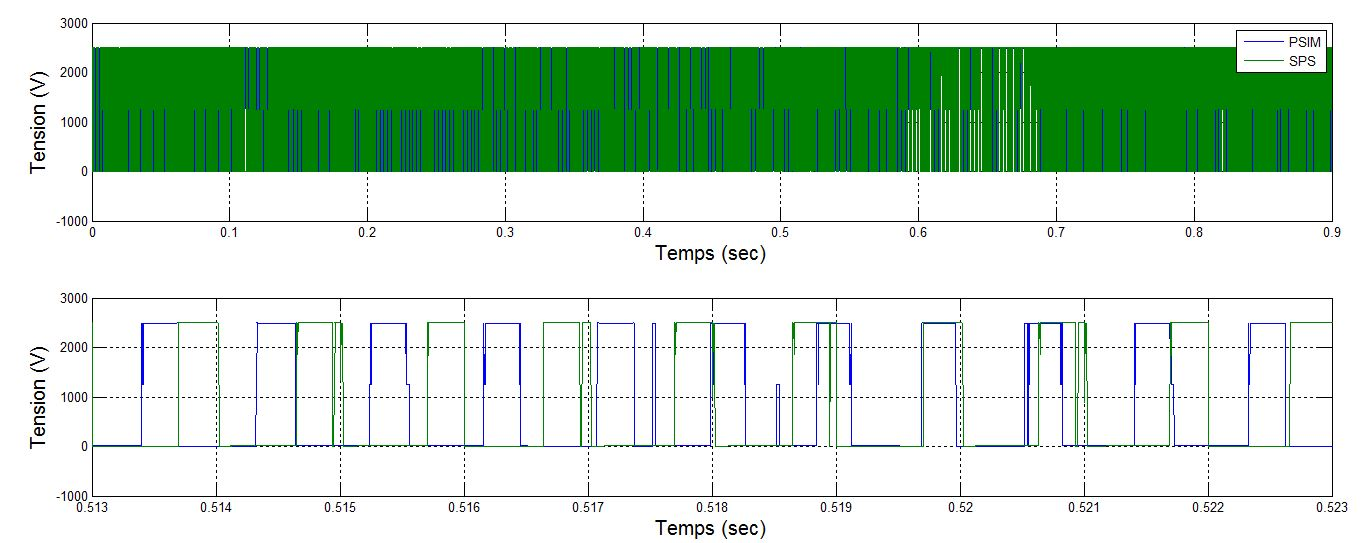
\includegraphics[scale=0.5]{Fig/DCPDCN/DCPTensionIGBT1u.jpg}
\caption{Tension aux bornes d'un IGBT sur PSIM et SPS pour un pas de calcul de 1$\mu$s pour le DCP/DCN}
\label{DC_IG_ten_1}
\end{figure}


\clearpage
\section{AFE 2 niveaux avec contrôle par hystérésis débitant sur une source idéale}
L'AFE (Active Front End) est un redresseur triphasé permettant de réguler le facteur de puissance à l'entrée du montage. La charge étant une source idéale pour cette simulation, il est possible d'en observer le fonctionnement dans les 4 quadrants. Ce convertisseur CA/CC est constitué de 6 interrupteurs, soit deux par bras. Ce système a pour fonction d'alimenter un bus CC et de maintenir sa tension à 5kV avec un facteur de puissance variable vu à l'entrée. Une méthode de contrôle par hystérésis est employée afin de réguler le courant (en amplitude et en phase) du côté du réseau. La figure \ref{AFE} est une représentation schématique de la commande de l'AFE débitant sur une source idéale. La figure \ref{circuit_AFE_IDEAL} présente le circuit électrique du convertisseur. Le tableau~\ref{p_AF_ID} présente les paramètres utilisés pour la simulation.

\begin{figure}[htb]
\centering
<<<<<<< HEAD
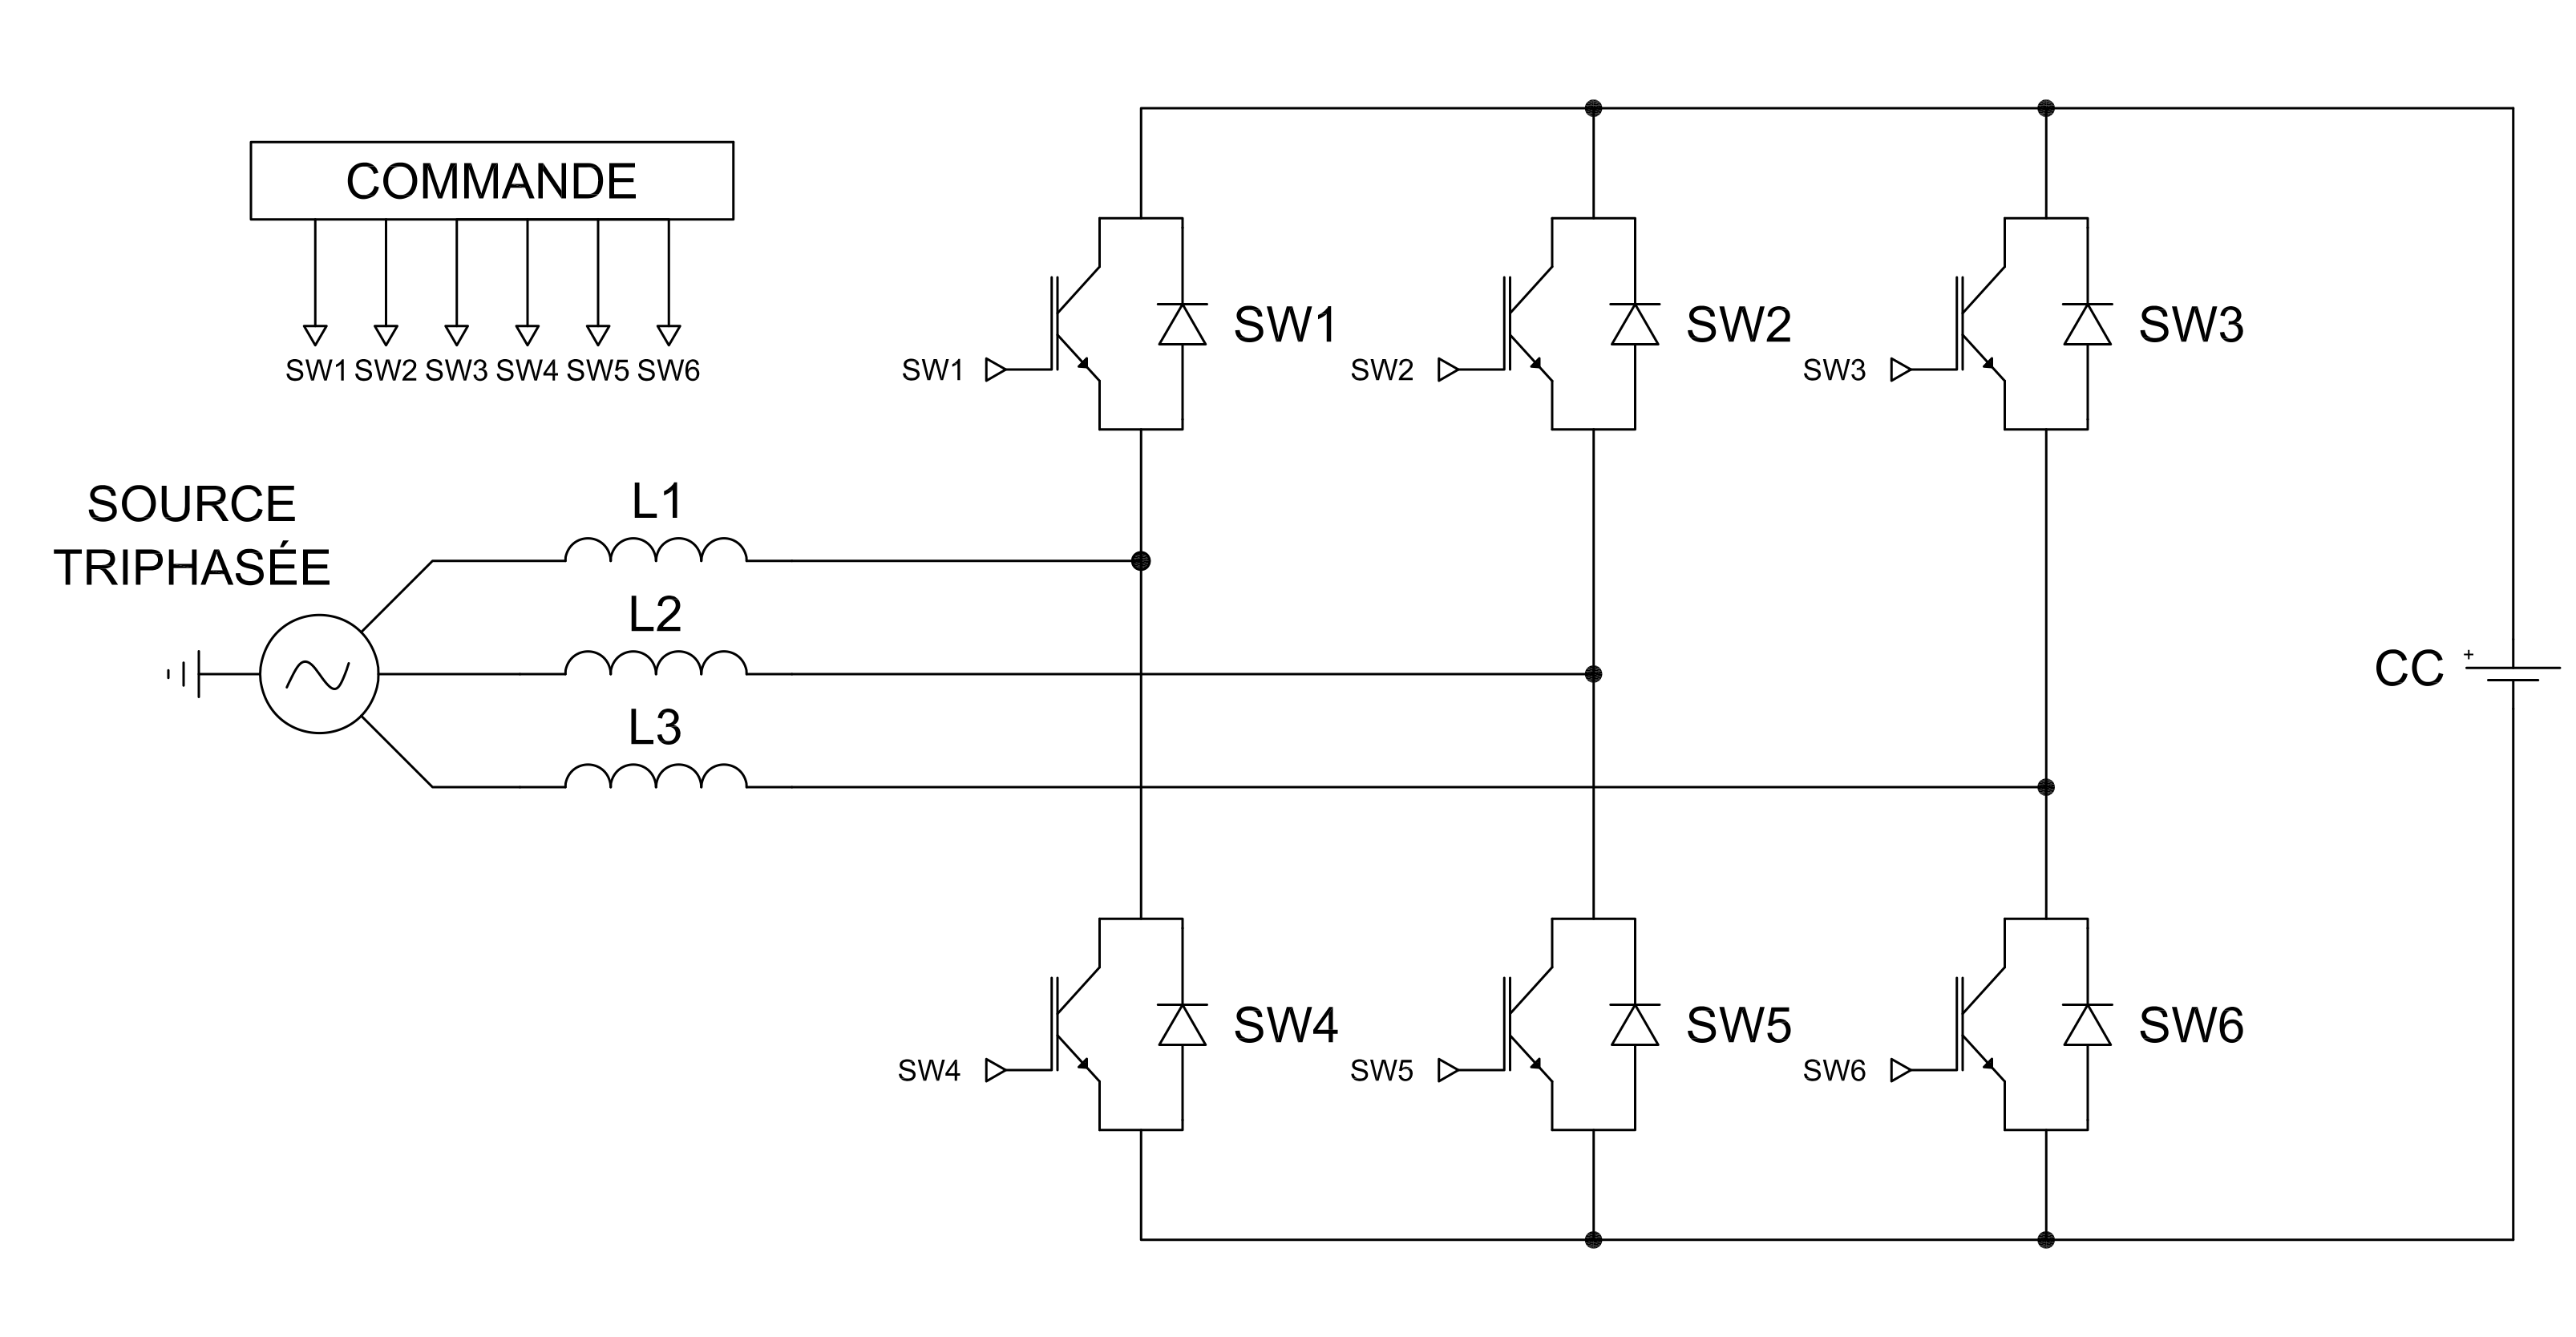
\includegraphics[scale=0.6]{Fig/AFE_IDEAL.png}
\caption{Circuit électrique de l'AFE 2 niveaux sur source parfaite}
\label{circuit_AFE_IDEAL}
=======
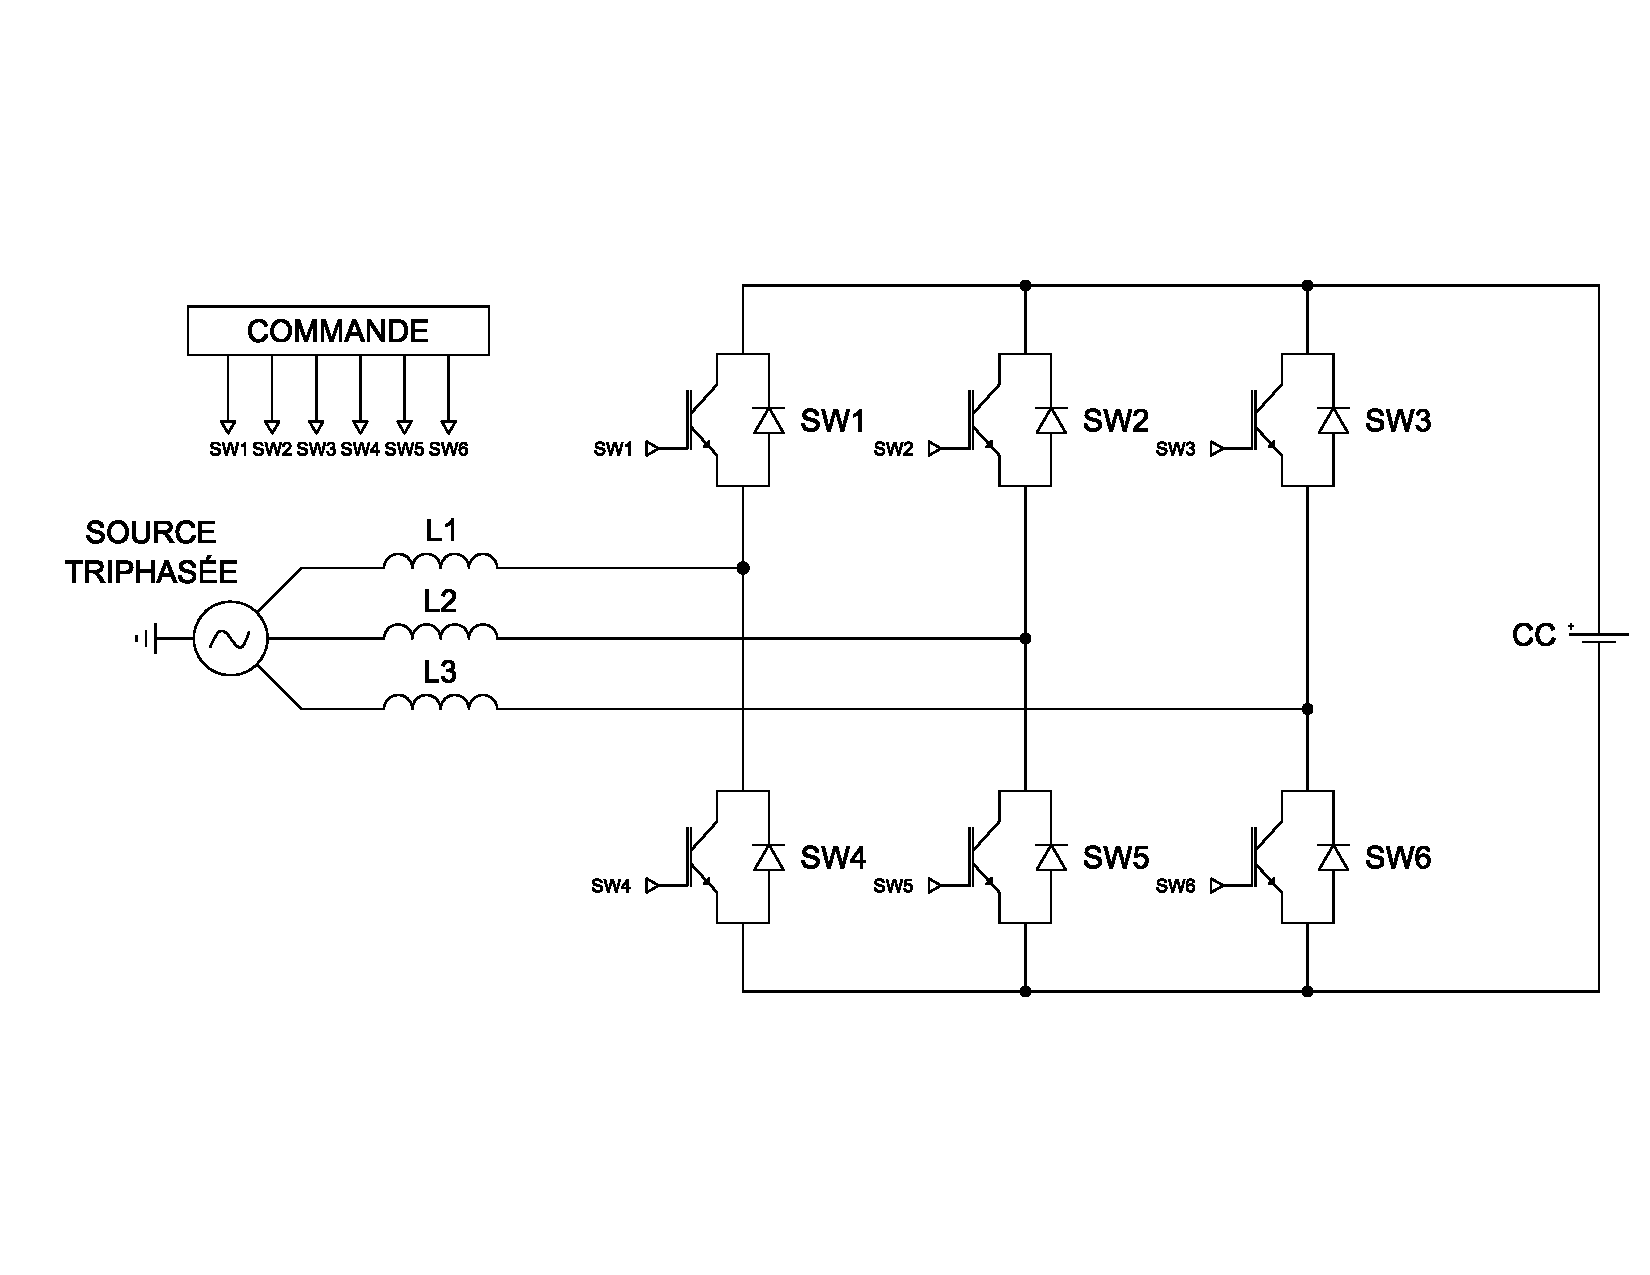
\includegraphics[scale=0.5]{Fig/AFEIDEAL/AFE_IDEAL.pdf}
\caption{Schéma bloc de l'AFE 2 niveau sur source parfaite avec régulation par hystérésis}
\label{AFE}
>>>>>>> FETCH_HEAD
\end{figure}


\begin{table}[htb]
\centering
\begin{tabular}{|l|c|} 
  \hline
  \textbf{Paramètre} & \textbf{Valeur}  \\
  \hline\hline
  Tension bus CC & 5000\\ \hline
  Courant référence & 1000A\\ \hline
  Seuil hystérésis & 450A\\ \hline
  Courant maximal à l'entrée& 1500A \\ \hline \hline
  \multicolumn{2}{|c|}{\textbf{IGBT}}\\ \hline
  Résistance interne & 0.001$\Omega$\\
  Résistance du snubber & 100k$\Omega$\\ \hline \hline
   \multicolumn{2}{|c|}{\textbf{PI de courant}}\\ \hline
  Gain proportionnel & 5 \\
  Gain intégrateur & 20 \\ \hline \hline
  \multicolumn{2}{|c|}{\textbf{PI de phase}}\\ \hline
  Gain proportionnel & 0.48 \\
  Gain intégrateur & 8 \\ \hline \hline
  \hline
\end{tabular}
\caption{Paramètres de simulation pour l'AFE débitant sur une source idéale}
\label{p_AF_ID}
\end{table}
\clearpage

\subsection{Vérification pour un pas de calcul de 1$\mu$s}
Cette section présente les résultats de simulation de l'AFE 2 niveaux avec contrôle par hystérésis, débitant sur une source idéale, pour un pas de calcul discret de 1$\mu$s. 


\begin{figure}[htb]
\centering
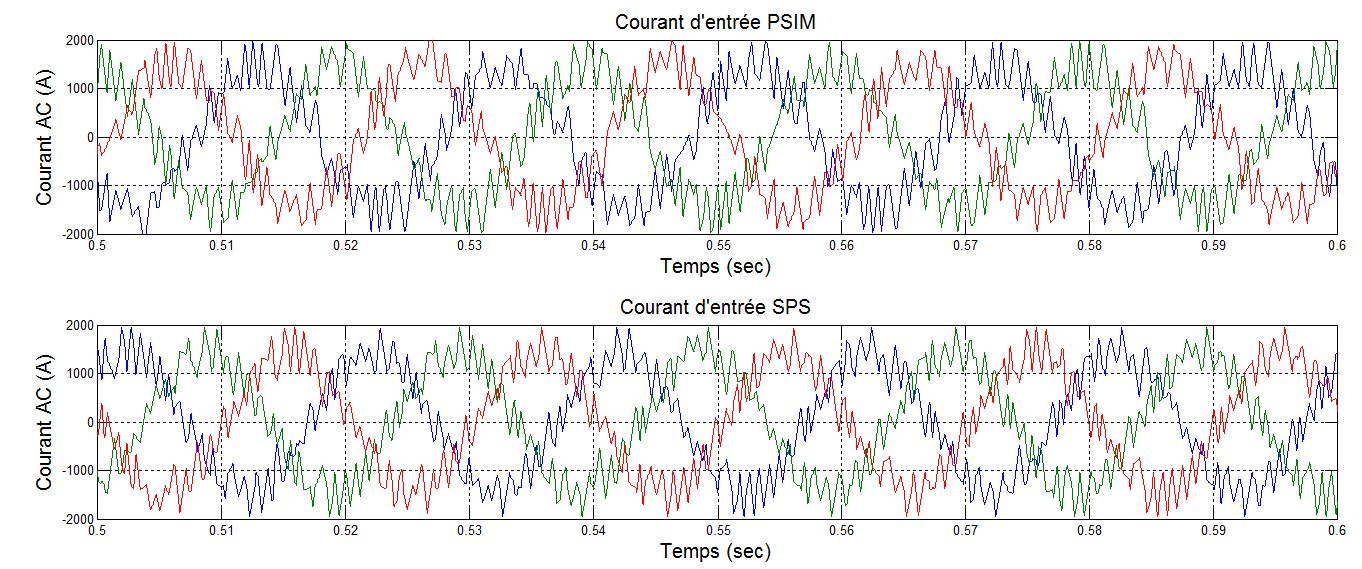
\includegraphics[scale=0.5]{Fig/AFEIDEAL/CourantAC.jpg}
\caption{Le courant d'entrée avec un pas de calcul de 1$\mu$s pour l'AFE 2 niveaux avec contrôle par hystérésis sur source idéale}
\label{AF_I_cou}
\end{figure}



\begin{figure}[htb]
\centering
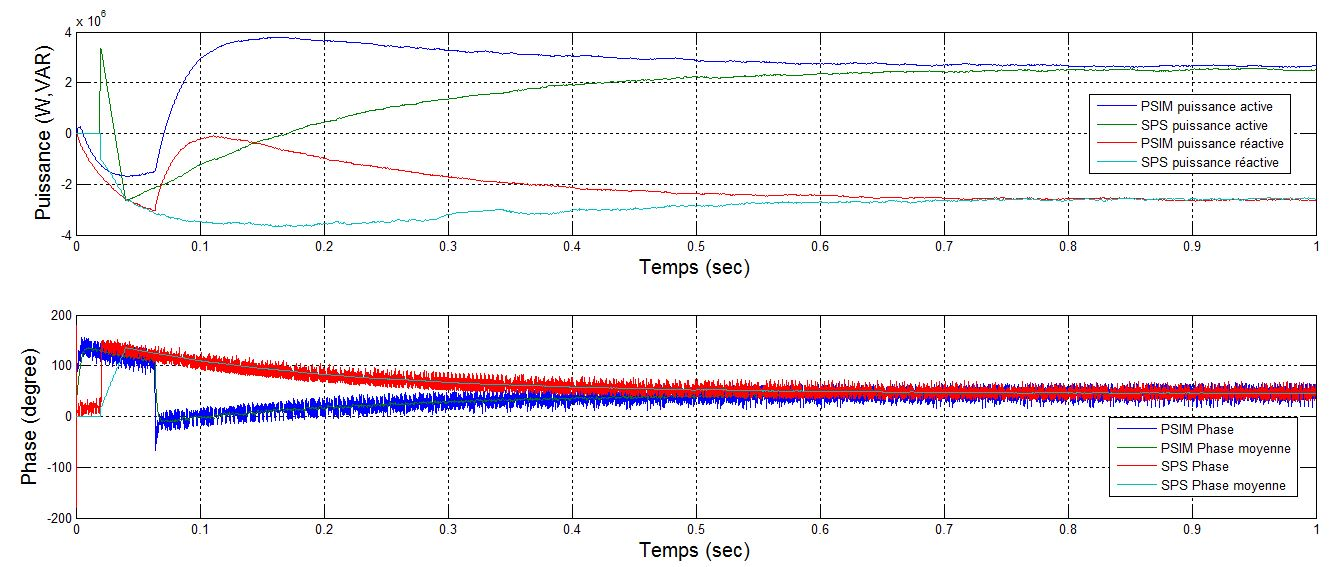
\includegraphics[scale=0.5]{Fig/AFEIDEAL/pui45.jpg}
\caption{Puissances active et réactive pour une courant déphasé de 45 degré pour un pas de calcul 1$\mu$s}
\label{AF_I_pui_45}
\end{figure}

\begin{figure}[htb]
\centering
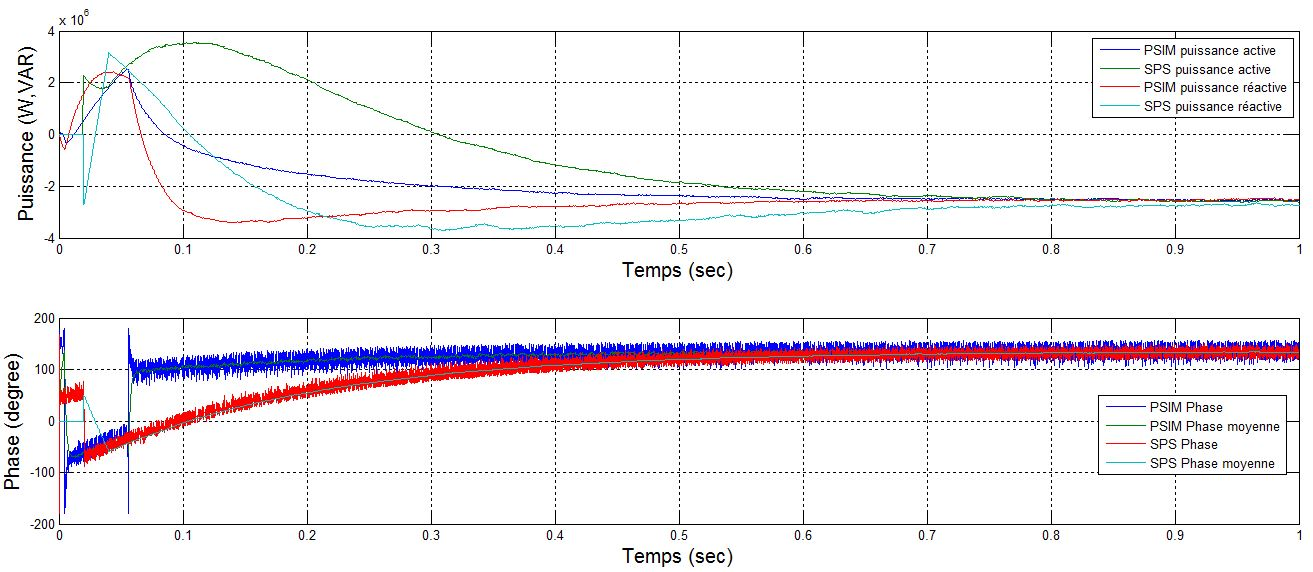
\includegraphics[scale=0.5]{Fig/AFEIDEAL/pui135.jpg}
\caption{Puissances active et réactive pour une courant déphasé de 135 degré pour un pas de calcul 1$\mu$s}
\label{AF_I_pui_135}
\end{figure}

\begin{figure}[htb]
\centering
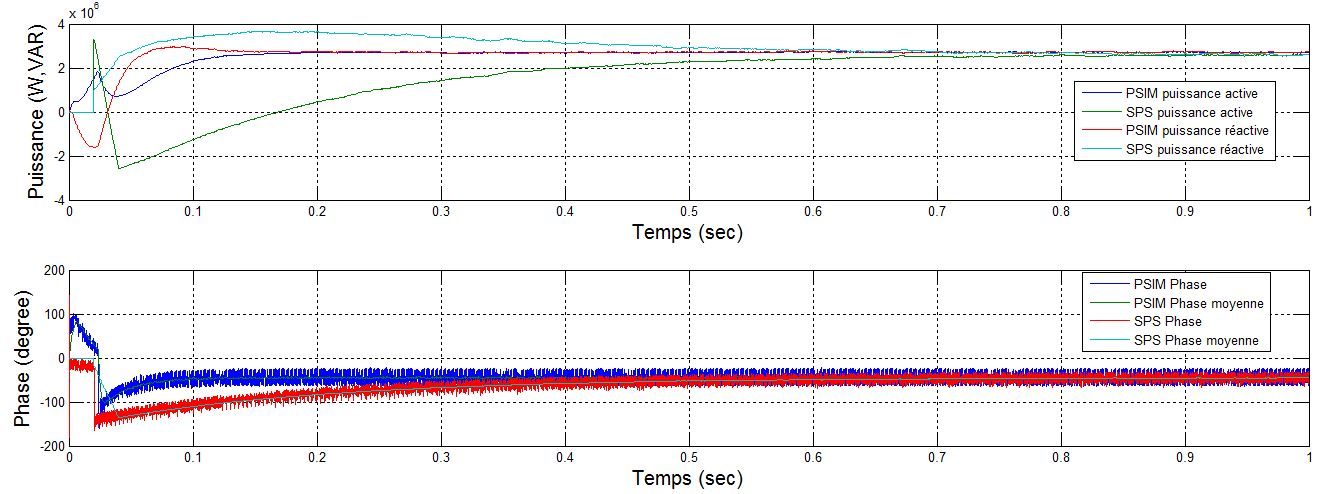
\includegraphics[scale=0.5]{Fig/AFEIDEAL/pui_45.jpg}
\caption{Puissances active et réactive pour une courant déphasé de -45 degré pour un pas de calcul 1$\mu$s}
\label{AF_I_pui__45}
\end{figure}

\begin{figure}[htb]
\centering
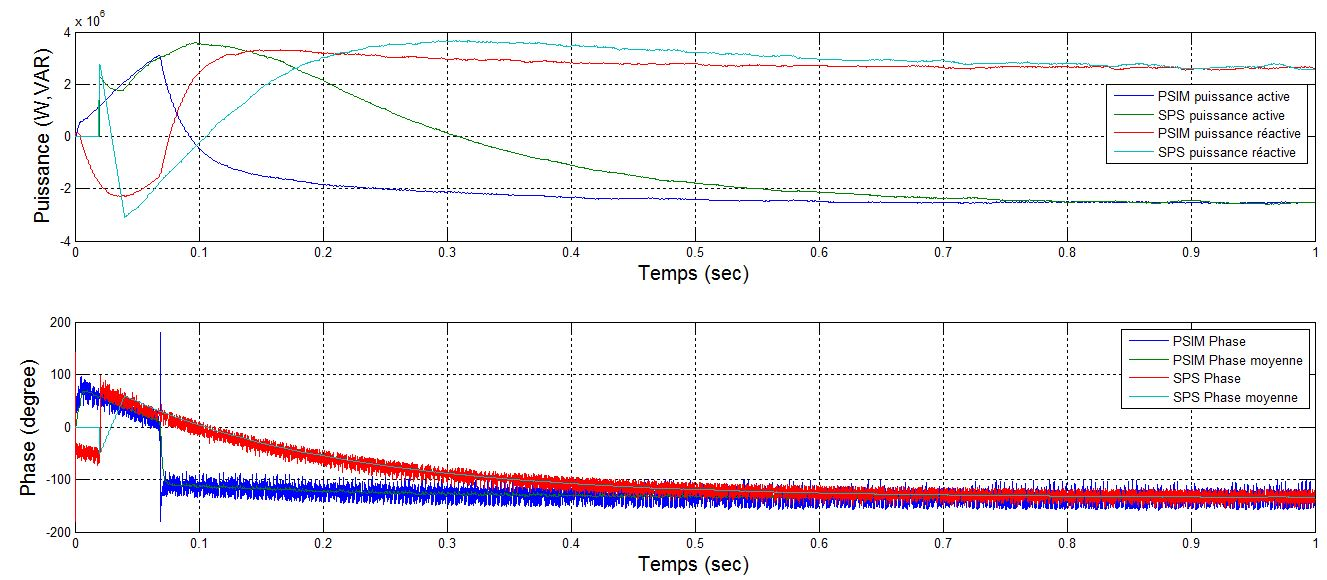
\includegraphics[scale=0.5]{Fig/AFEIDEAL/pui_135.jpg}
\caption{Puissances active et réactive pour une courant déphasé de -135 degré pour un pas de calcul 1$\mu$s}
\label{AF_I_pui__135}
\end{figure}


\clearpage
\section{AFE 2 niveaux avec contrôle par hystérésis débitant sur une charge RC}
Le modèle de redresseur 2 niveaux AFE avec contrôle par hystérésis débitant sur une charge RC est le même que celui présenté dans la figure \ref{AFE}. Le circuit du convertisseur est présenté à la figure \ref{circuit_AFE_2L_RC}. La source idéale du montage précédent est remplacée par une charge RC, composée d'une résistance de 9.26$\Omega$ et d'un condensateur initialement chargé à 5000V, d'une capacité de 330mF. De plus, contrairement au montage précédent, il n'y a plus de rétroaction sur l'angle du courant. L'angle de la référence de courant est en phase avec la tension du réseau (pour un fonctionnement à facteur unitaire). La figure \ref{fft_RC} représente le calcul de transformée de Fourier discrète (fft) d'une phase du courant d'entrée. Les paramètres de l'hystérésis ont été ajustés afin que la fréquence de commutation (qui glisse avec cette méthode de commande), soit proche de 1kHz. Le tableau \ref{p_AF_RC} présente les paramètres utilisés pour l'AFE 2 niveaux débitant sur une charge RC.

\begin{figure}[htb]
\centering
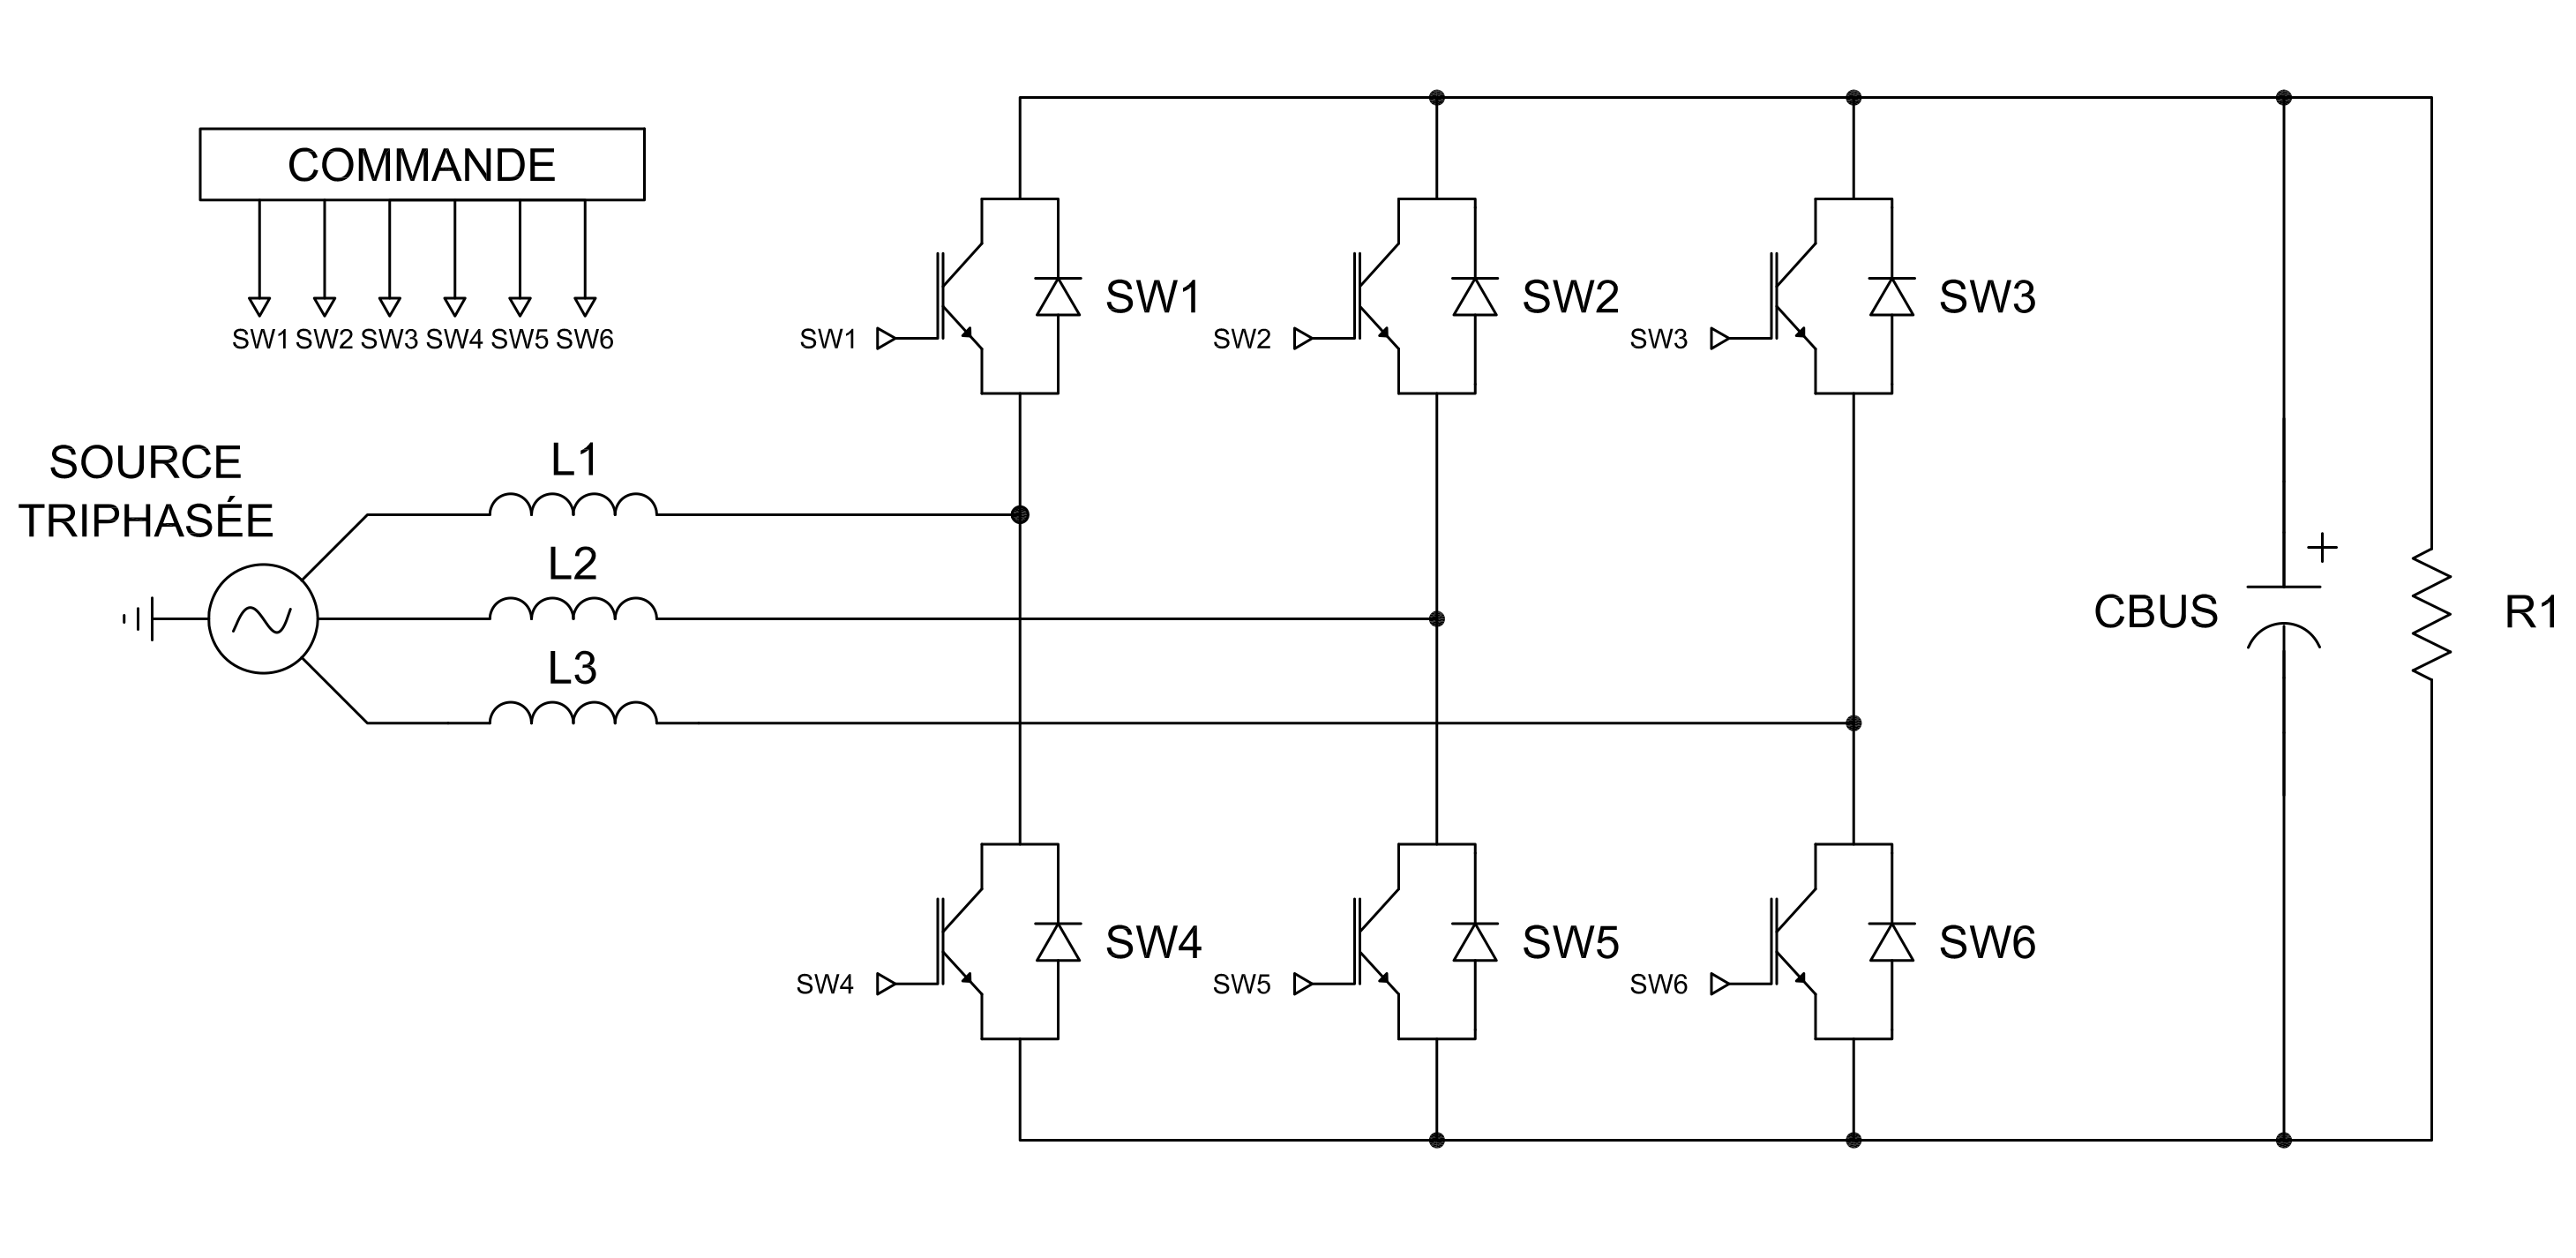
\includegraphics[scale=0.6]{Fig/AFE_2L_RC.png}
\caption{Circuit électrique de l'AFE 2 niveaux sur une charge RC}
\label{circuit_AFE_2L_RC}
\end{figure}


\begin{figure}[htb]
\centering
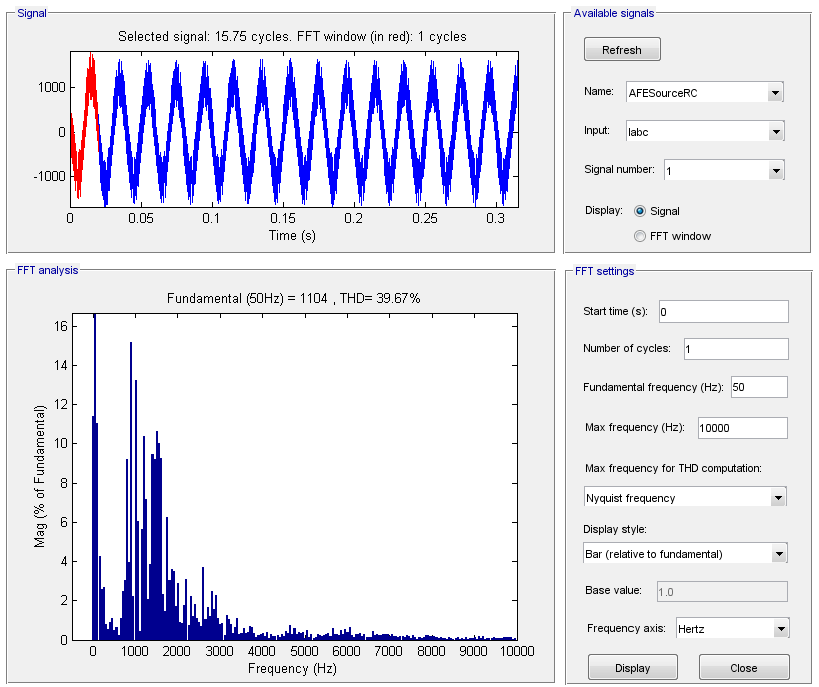
\includegraphics[scale=0.5]{Fig/AFERC/FFTAnalysisToolResult5u.png}
\caption{La transformée de Fourier discrète (fft) du courant d'entrée à 1$\mu$s}
\label{fft_RC}
\end{figure}


\begin{figure}[htb]
\centering
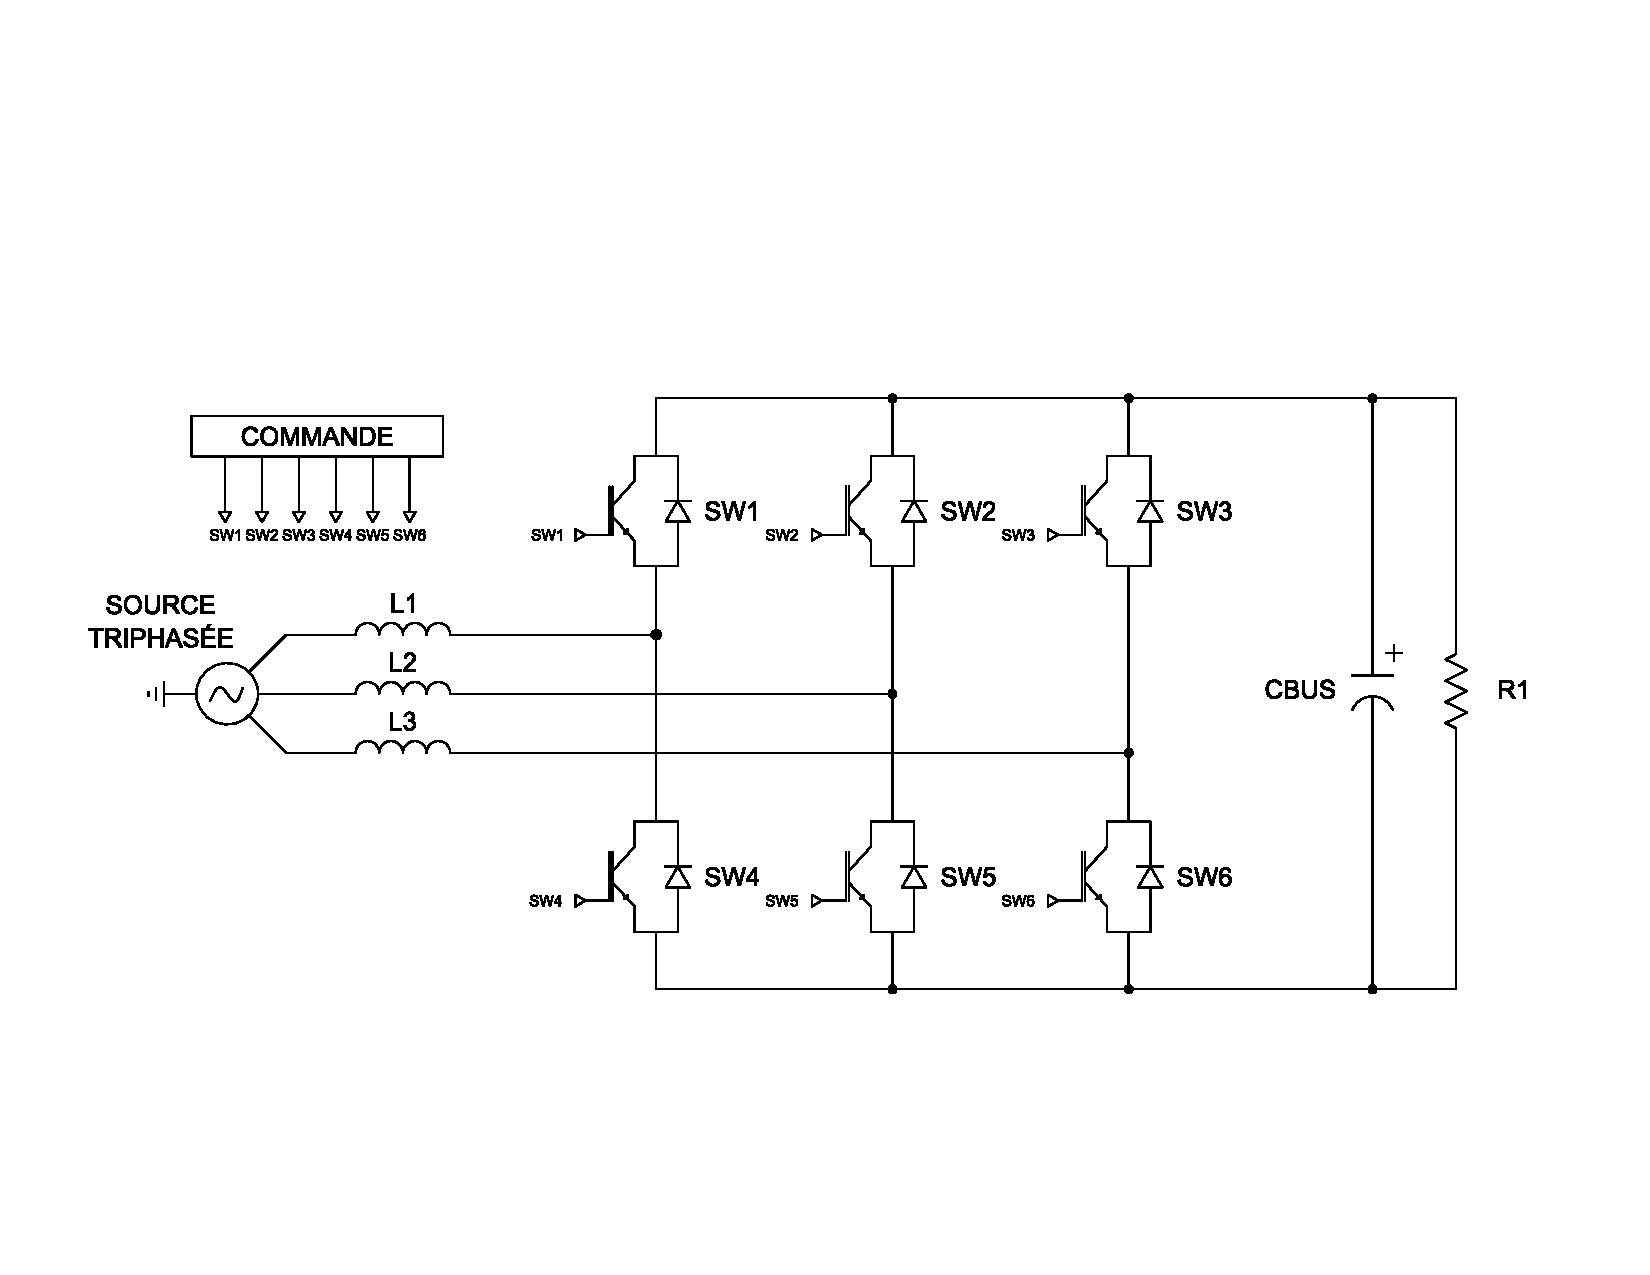
\includegraphics[scale=0.6]{Fig/AFERC/AFE_2L_RC.pdf}
\caption{Circuit électrique d'un AFE 2 niveaux sur charge RC}
\label{AFE_RC}
\end{figure}

\begin{table}[htb]
\centering
\begin{tabular}{|l|c|} 
  \hline
  \textbf{Paramètre} & \textbf{Valeur}  \\
  \hline\hline
  Tension de référence CC & 5000 V\\ \hline
  Seuil hystérésis & 450 A\\ \hline
  Courant maximal à l'entrée& 1500 A \\ \hline \hline
  \multicolumn{2}{|c|}{\textbf{IGBT}}\\ \hline
  Résistance interne & 0.001 $\Omega$\\
  Résistance du snubber & 100k $\Omega$\\ \hline \hline
   \multicolumn{2}{|c|}{\textbf{PI courant}}\\ \hline
  Gain proportionnel & 5 \\
  Gain intégrateur & 20 \\ \hline \hline
  \multicolumn{2}{|c|}{\textbf{Charge}}\\ \hline
  Résistance & 9.26 $\Omega$ \\
  Capacité d'entrée & 330 mF\\
  \hline
\end{tabular}
\caption{Paramètres de simulation pour l'AFE 2 niveaux avec contrôle par hystérésis débitant sur charge RC}
\label{p_AF_RC}
\end{table}

\clearpage

\subsection{Vérification pour un pas de calcul de 1$\mu$s}
Cette section présente les résultats de simulation de l'AFE 2 niveaux avec contrôle pas hystérésis sur charge RC, pour un pas de calcul discret de 1$\mu$s. 




\begin{figure}[htb]
\centering
\includegraphics[scale=0.5]{Fig/AFERC/cour_al.jpg}
\caption{Le courant d'entré à 1$\mu$s pour l'AFE sur charge RC}
\label{AF_RC_cou}
\end{figure}




\begin{figure}[htb]
\centering
\includegraphics[scale=0.5]{Fig/AFERC/vch.jpg}
\caption{La tension à la charge à 1$\mu$s pour l'AFE sur charge RC}
\label{AF_RC_ten}
\end{figure}



\begin{figure}[htb]
\centering
\includegraphics[scale=0.5]{Fig/AFERC/IGBT.jpg}
\caption{La tension et le courant au bornes d'un IGBT à 1$\mu$s pour l'AFE sur charge RC}
\label{AF_RC_igbt}
\end{figure}

\clearpage
\section{AFE 3 niveaux NPC avec contrôle par MLI}
L'AFE 3 niveaux NPC avec contrôle par MLI est composé de 12 interrupteurs IGBT ainsi que de 6 diodes de point milieu. Il représente la version finale du sous-système de l'AFE. La méthode de commande implantée diffère de celle implantée au CERN qui utilise une transformation de Park afin de simplifier le contrôle. Le circuit électrique de l'AFE 3 niveaux sur charge RC est présenté à la figure \ref{circuit_AFE_3L_RC}. Le tableau \ref{p_AF_3level} présente les paramètres utilisés avec l'AFE 3 niveaux NPC.

\begin{figure}[htb]
\centering
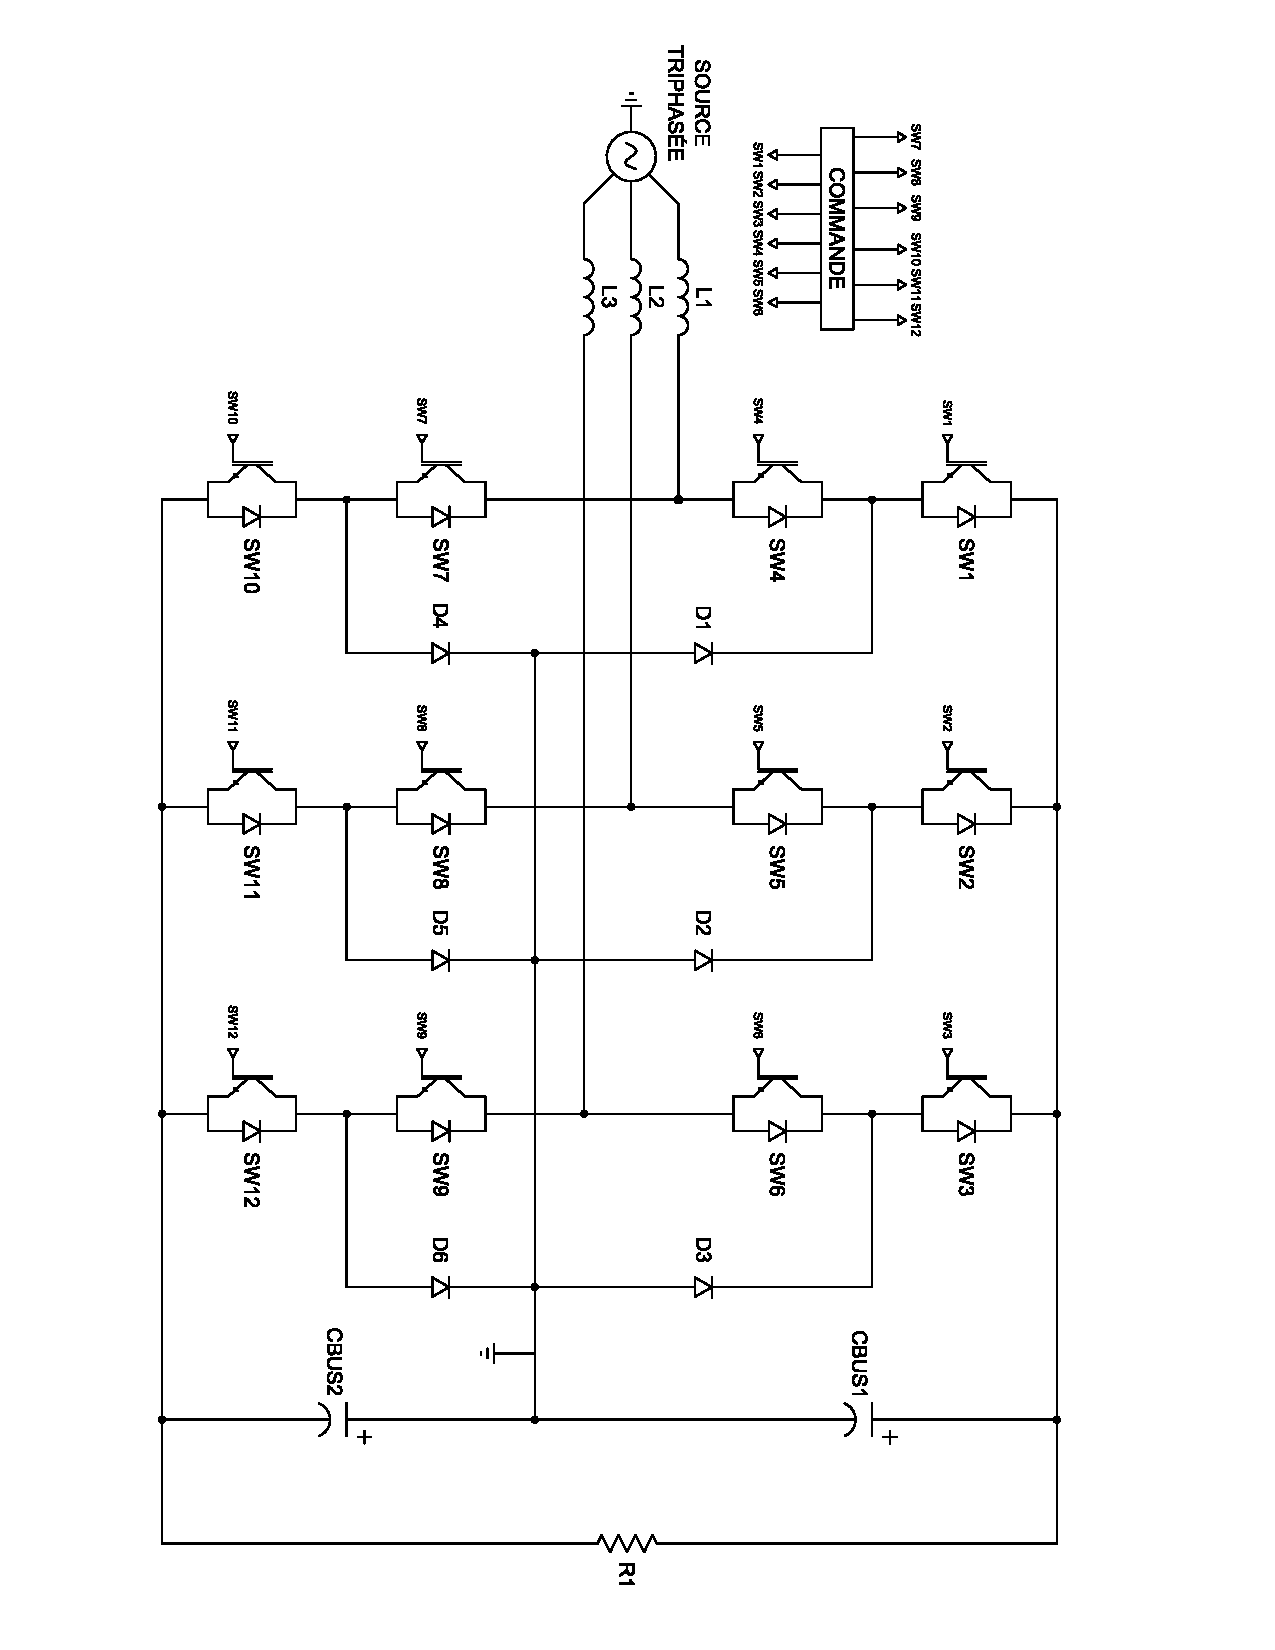
\includegraphics[scale=0.6]{Fig/AFE3LEVEL/AFE_3L_RC.pdf}
\caption{Circuit électrique d'un AFE 3 niveaux sur charge RC}
\label{AFE_3L}
\end{figure}

\begin{table}[htb]
\centering
\begin{tabular}{|l|c|} 
  \hline
  \textbf{Paramètre} & \textbf{Valeur}  \\
  \hline\hline
  Tension référence CC & 5000 V\\ \hline
  Fréquence de modulation & 1000 Hz \\ \hline
  Courant maximal à l'entrée& 1500 A \\ \hline \hline
  \multicolumn{2}{|c|}{\textbf{IGBT}}\\ \hline
  Résistance interne & 0.001 $\Omega$\\
  Résistance du snubber & 100k $\Omega$\\ \hline \hline
   \multicolumn{2}{|c|}{\textbf{PI courant}}\\ \hline
  Gain proportionnel & 5 \\
  Gain intégrateur & 20 \\ \hline \hline
  \multicolumn{2}{|c|}{\textbf{PI commande}}\\ \hline
  Rapport cyclique maximal & 0.95\\
  Gain proportionnel & 1.5611 \\
  Gain intégrateur & 24.6 \\ \hline \hline
  \multicolumn{2}{|c|}{\textbf{Charge}}\\ \hline
  Résistance & 9.26 $\Omega$ \\
  Capacité d'entrée & 330 mF\\
  \hline
\end{tabular}
\caption{Paramètres de simulation pour l'AFE 3 niveaux NPC avec contrôle par MLI}
\label{p_AF_3level}
\end{table}

\begin{figure}[htb]
\centering
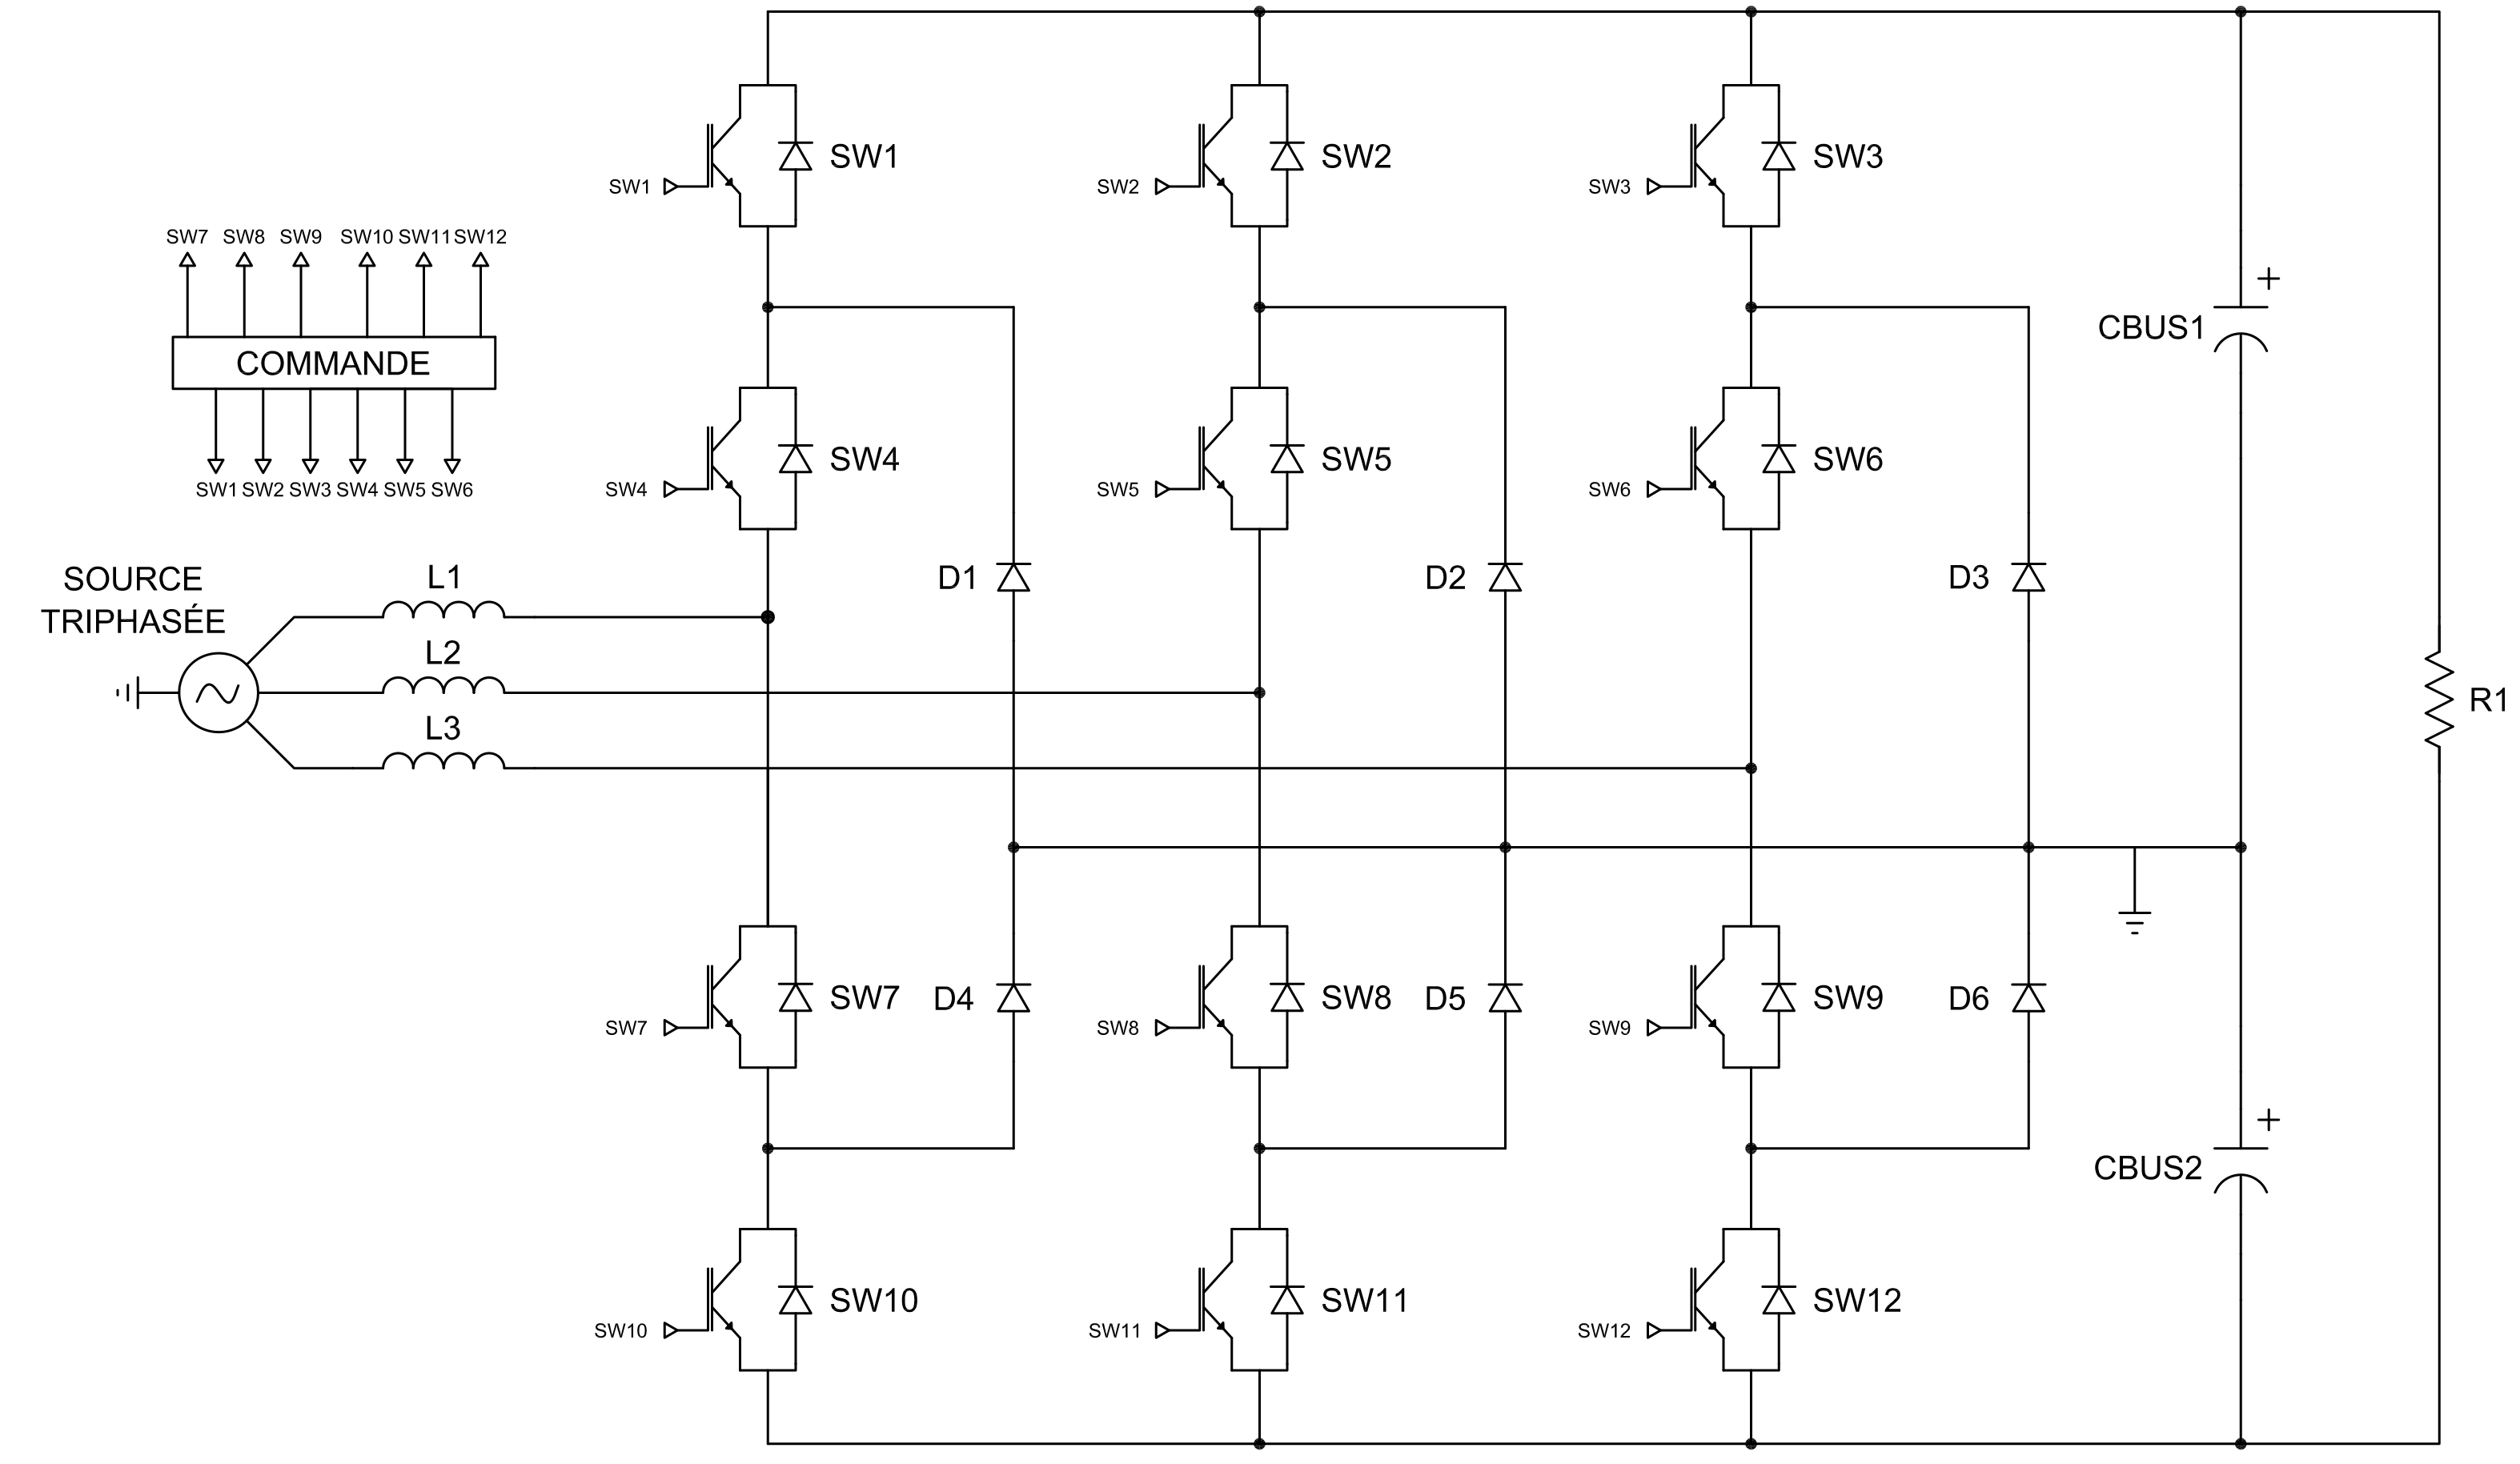
\includegraphics[scale=0.6]{Fig/AFE_3L_RC.png}
\caption{Circuit électrique de l'AFE 3 niveaux sur charge RC}
\label{circuit_AFE_3L_RC}
\end{figure}


\clearpage
\subsection{Vérification pour un pas de calcul de 1$\mu$s}
Cette section présente les courbes d'intérêt pour la simulation de l'AFE 3 niveaux NPC avec contrôle par MLI, pour un pas de 1$\mu$s. 

\begin{figure}[htb]
\centering
\includegraphics[scale=0.5]{Fig/AFE3LEVEL/1u/cour_al.jpg}
\caption{Le courant d'entrée pour un pas de calcul de 1$\mu$s, pour l'AFE 3 niveaux}
\label{AF_3_cou}
\end{figure}


\begin{figure}[htb]
\centering
\includegraphics[scale=0.5]{Fig/AFE3LEVEL/1u/vch.jpg}
\caption{La tension à la charge pour un pas de calcul de 1$\mu$s, pour l'AFE 3 niveaux}
\label{AF_3_vch}
\end{figure}


\begin{figure}[htb]
\centering
\includegraphics[scale=0.5]{Fig/AFE3LEVEL/1u/IGBT.jpg}
\caption{La tension et le courant au niveau d'un IGBT pour un pas de calcul de 1$\mu$s, pour l'AFE 3 niveaux}
\label{AF_3_IGBT}
\end{figure}

\begin{figure}[htb]
\centering
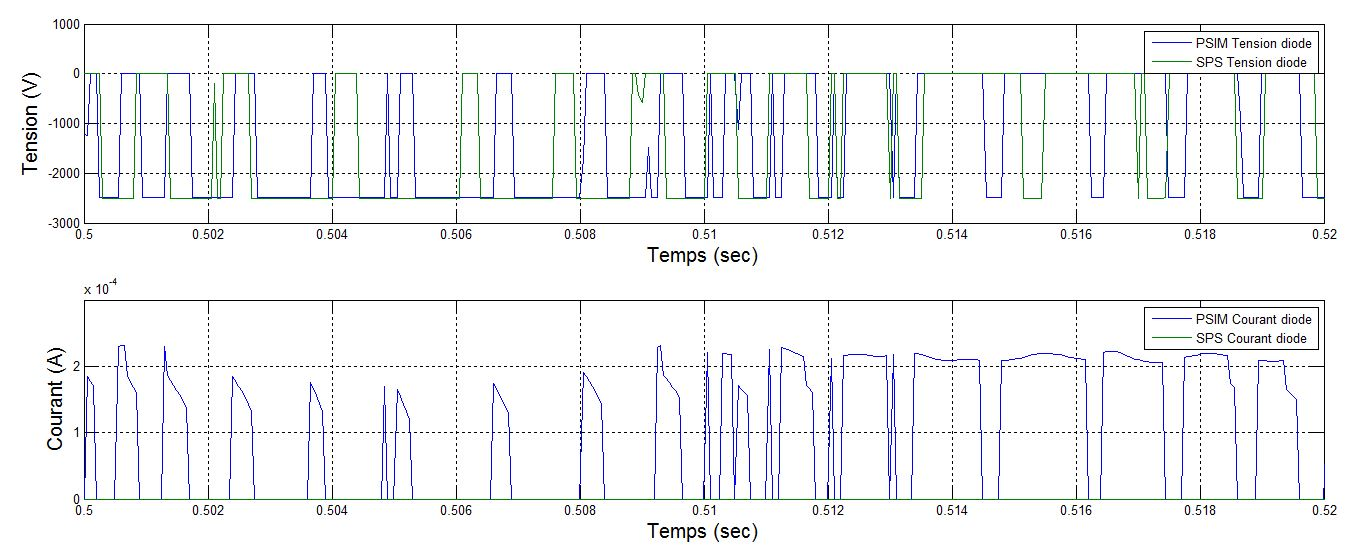
\includegraphics[scale=0.5]{Fig/AFE3LEVEL/1u/DIODE.jpg}
\caption{La tension et le courant au niveau d'une diode pour un pas de calcul de 1$\mu$s, pour l'AFE 3 niveaux}
\label{AF_3_DIODE}
\end{figure}


\clearpage
\section{AFE 2 niveaux avec contrôle par hystérésis et hacheur 4 quadrants à 4 IGBT}
Cette section présente les résultat de simulations obtenus sur PSIM et SPS pour l'AFE 2 niveaux avec contrôle par hystérésis et hacheur 4 quadrants à 4 IGBT. Le circuit électronique des 2 convertisseurs est présenté à la figure \ref{circuit_H4Q_AFE_2L_RC}. Le tableau \ref{p_AF_hash} présente les paramètres utilisés dans les simulations.

\begin{figure}[htb]
\centering
<<<<<<< HEAD
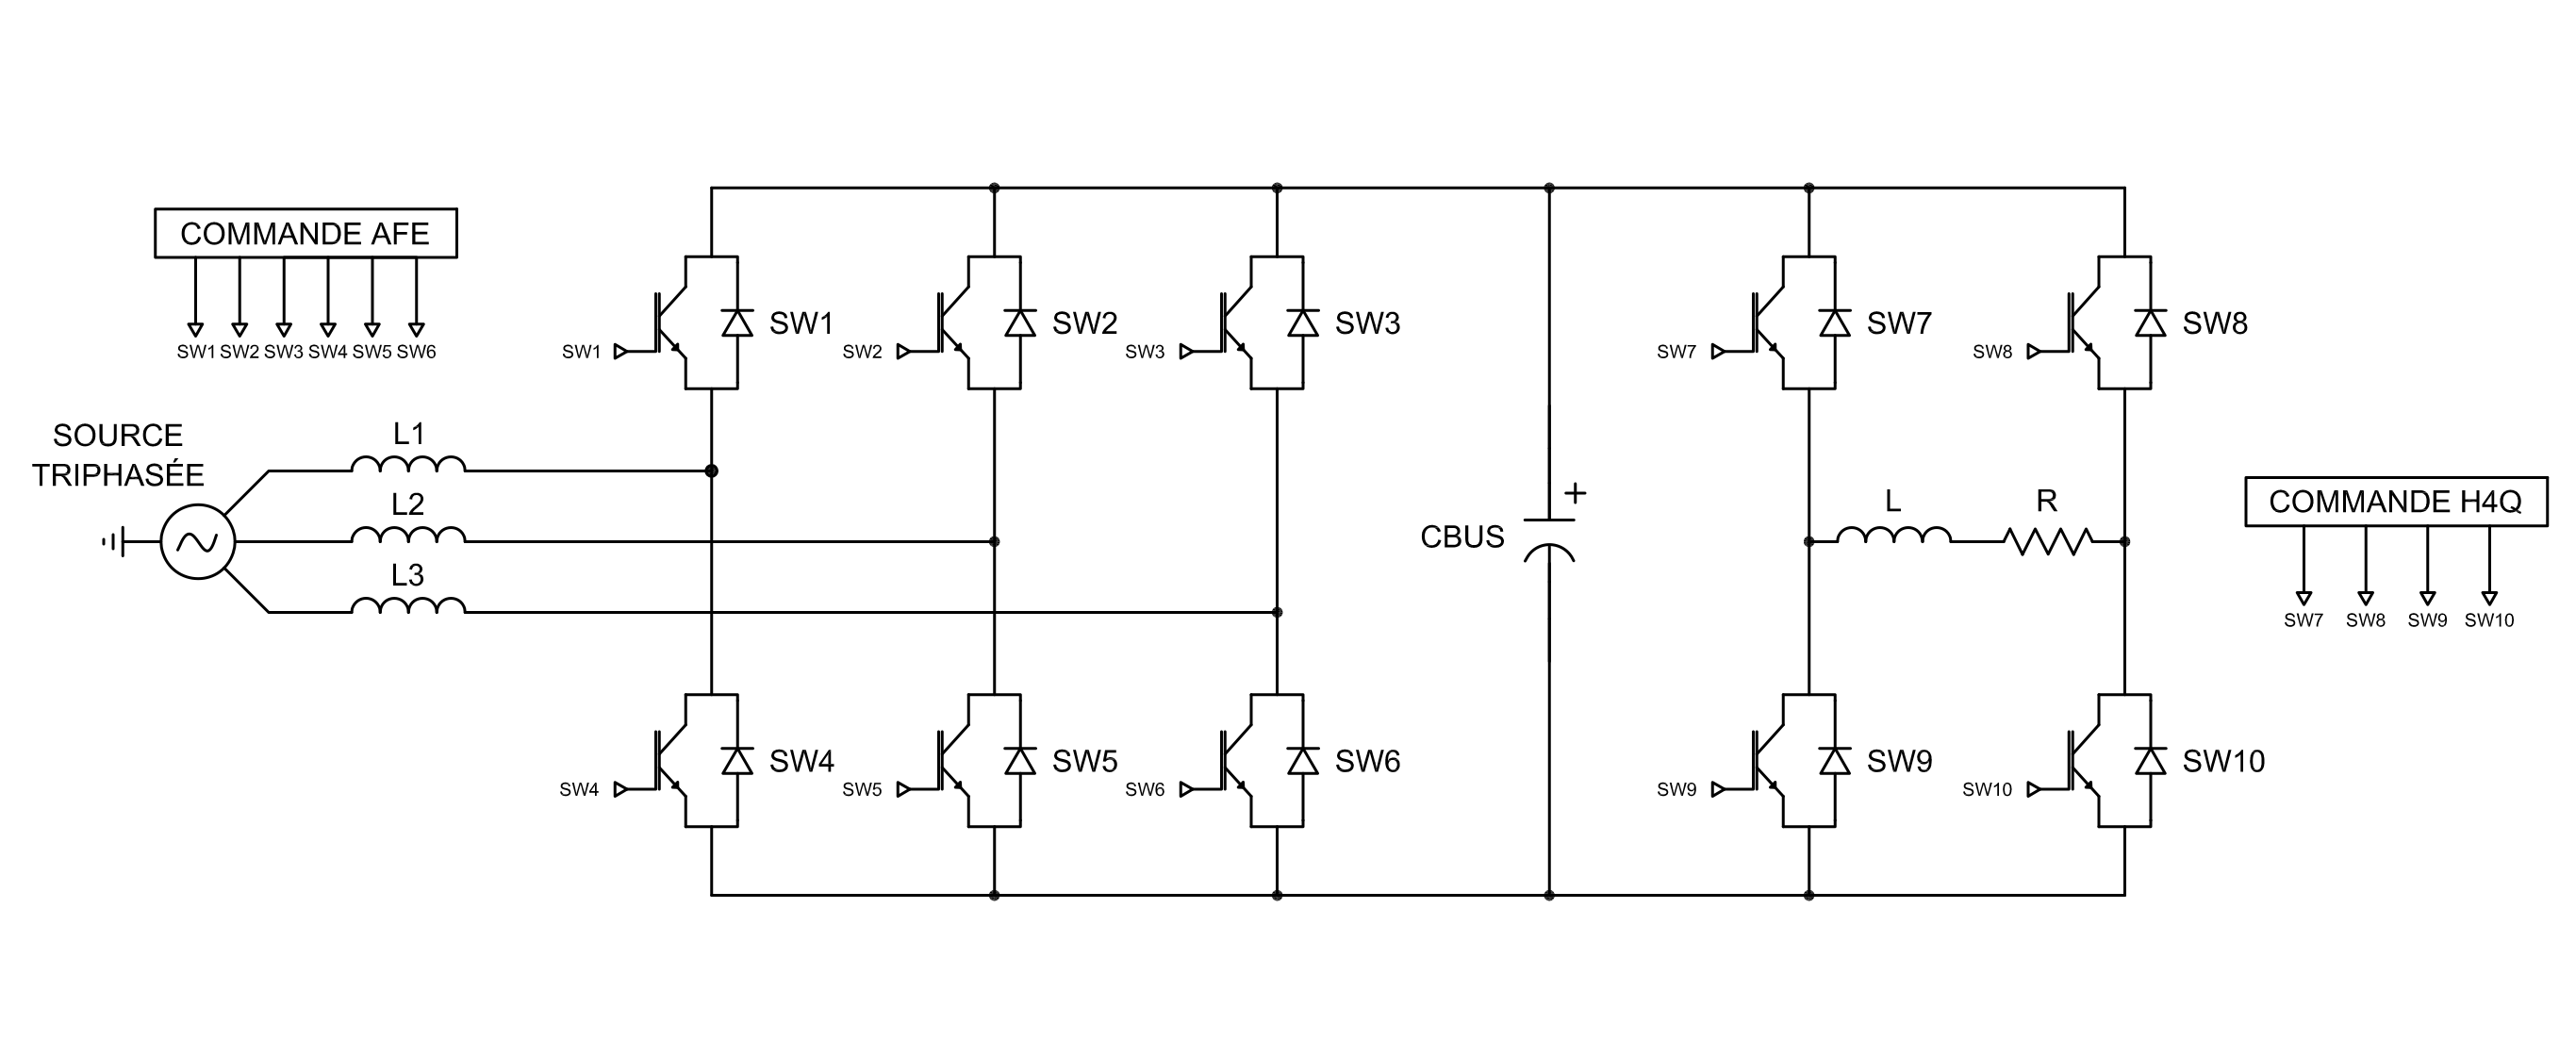
\includegraphics[scale=0.6]{Fig/H4Q_AFE_2L_RC.png}
\caption{Circuit électrique de l'AFE 2 niveaux avec contrôle par hystérésis et hacheur 4 quadrants à 4 IGBT}
\label{circuit_H4Q_AFE_2L_RC}
=======
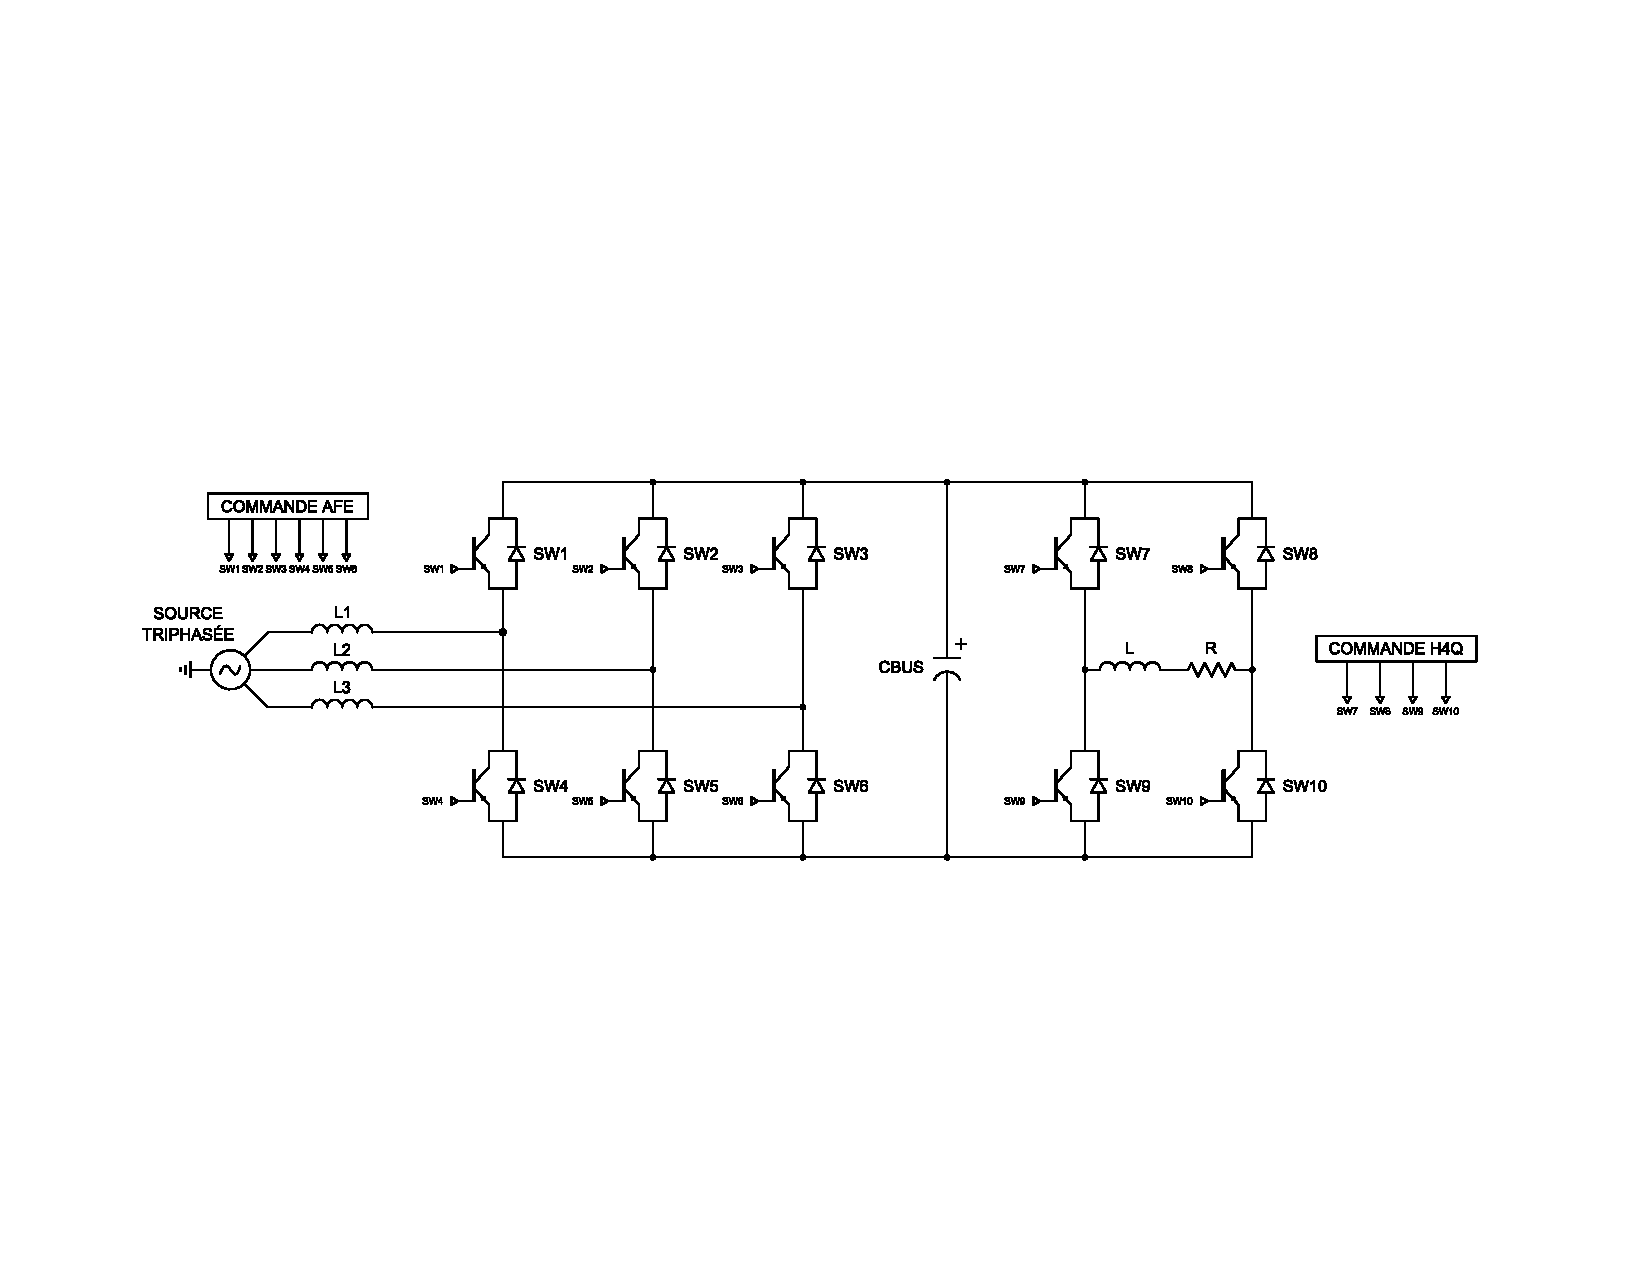
\includegraphics[scale=0.7]{Fig/Hach_AFE/H4Q_AFE_2L_RC.pdf}
\caption{Circuit électrique de l'implantation de l'AFE 2 niveaux et du hacheur 4 quadrants}
\label{AF_DC}
>>>>>>> FETCH_HEAD
\end{figure}



\begin{table}[htb]
\centering
\begin{tabular}{|l|c|} 
  \hline
  \textbf{Paramètre} & \textbf{Valeur}  \\
  \hline\hline \hline
  \multicolumn{2}{|c|}{\textbf{AFE 2 niveaux}}\\ \hline \hline 
  Tension référence CC & 5000 V\\ \hline
  Seuil hystérésis & 450A\\ \hline
  Courant maximal à l'entrée& 1500A \\ \hline \hline
  \multicolumn{2}{|c|}{\textbf{IGBT AFE}}\\ \hline
  Résistance interne & 0.001 $\Omega$\\
  Résistance du snubber & 100k $\Omega$\\ \hline \hline
   \multicolumn{2}{|c|}{\textbf{PI courant AFE}}\\ \hline
  Gain proportionnel & 5 \\
  Gain intégrateur & 20 \\ \hline \hline
  \multicolumn{2}{|c|}{\textbf{Bus CC}}\\ \hline
  Capacité d'entrée & 330 mF\\
  \hline \hline \hline
  
  \multicolumn{2}{|c|}{\textbf{Hacheur 4 quadrants}}\\ \hline \hline
  Fréquence de modulation & 1000 Hz\\ \hline
  Rapport cyclique maximal & 0.95 \\ \hline \hline
  \multicolumn{2}{|c|}{\textbf{IGBT hacheur}}\\ \hline
  Résistance interne & 0.001 $\Omega$\\
  Résistance du snubber & 100k $\Omega$\\ \hline \hline
   \multicolumn{2}{|c|}{\textbf{PI hacheur}}\\ \hline
  Gain proportionnel & 0.071 \\
  Gain intégrateur & 50 \\ \hline \hline
  \multicolumn{2}{|c|}{\textbf{Charge}}\\ \hline
  Résistance & 0.28 $\Omega$\\
  Inductance & 0.1 H\\
  \hline
\end{tabular}
\caption{Paramètres de simulation pour l'hacheur 4 quadrants à 4 interrupteurs avec l'AFE 2 niveaux}
\label{p_AF_hash}
\end{table}
\clearpage

\subsubsection{Vérification pour un pas de calcul de 1$\mu$s}
Cette section présente les résultats de simulation pour l'hacheur 4 quadrants à 4 interrupteurs avec l'AFE 2 niveaux sur PSIM et sur SPS, pour un pas de calcul discret de 1$\mu$s. 


\begin{figure}[htb]
\centering
\includegraphics[scale=0.5]{Fig/Hach_AFE/1u/cour_al.jpg}
\caption{Le courant d'entré à 1$\mu$s section AFE}
\label{AF_HA_cou1}
\end{figure}


\begin{figure}[htb]
\centering
\includegraphics[scale=0.5]{Fig/Hach_AFE/1u/ten_bus.jpg}
\caption{La tension au bus CC à 1$\mu$s section AFE}
\label{AF_HA_vch1}
\end{figure}



\begin{figure}[htb]
\centering
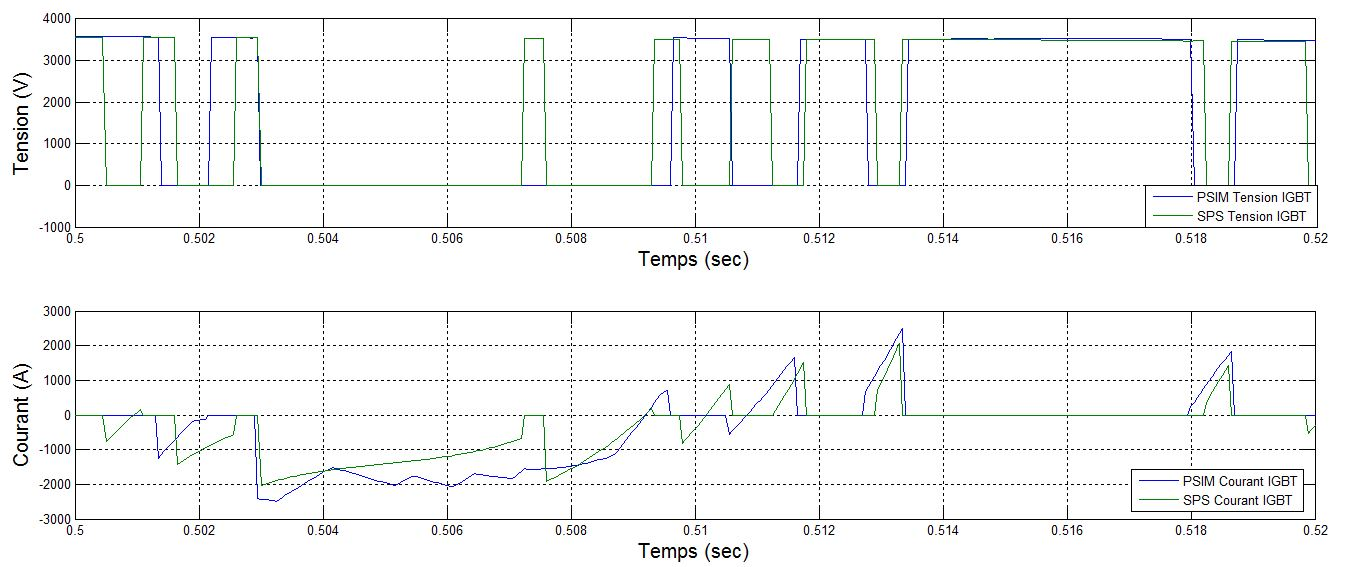
\includegraphics[scale=0.5]{Fig/Hach_AFE/1u/IGBT_AFE.jpg}
\caption{La tension et le courant au niveau d'un IGBT à 1$\mu$s au niveau de l'AFE}
\label{AF_HA_IGBT1}
\end{figure}


\begin{figure}[htb]
\centering
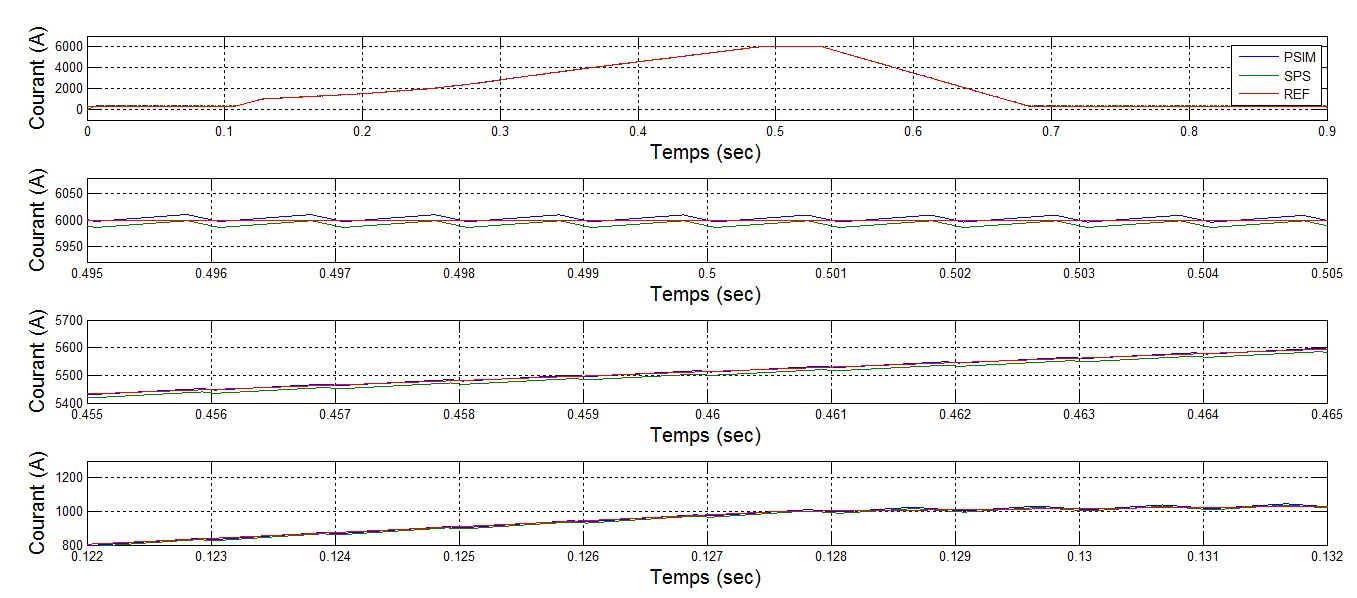
\includegraphics[scale=0.5]{Fig/Hach_AFE/1u/hach_cou_ch.jpg}
\caption{Le courant au niveau de la charge à 1$\mu$s}
\label{AF_HA_CHA1}
\end{figure}



\begin{figure}[htb]
\centering
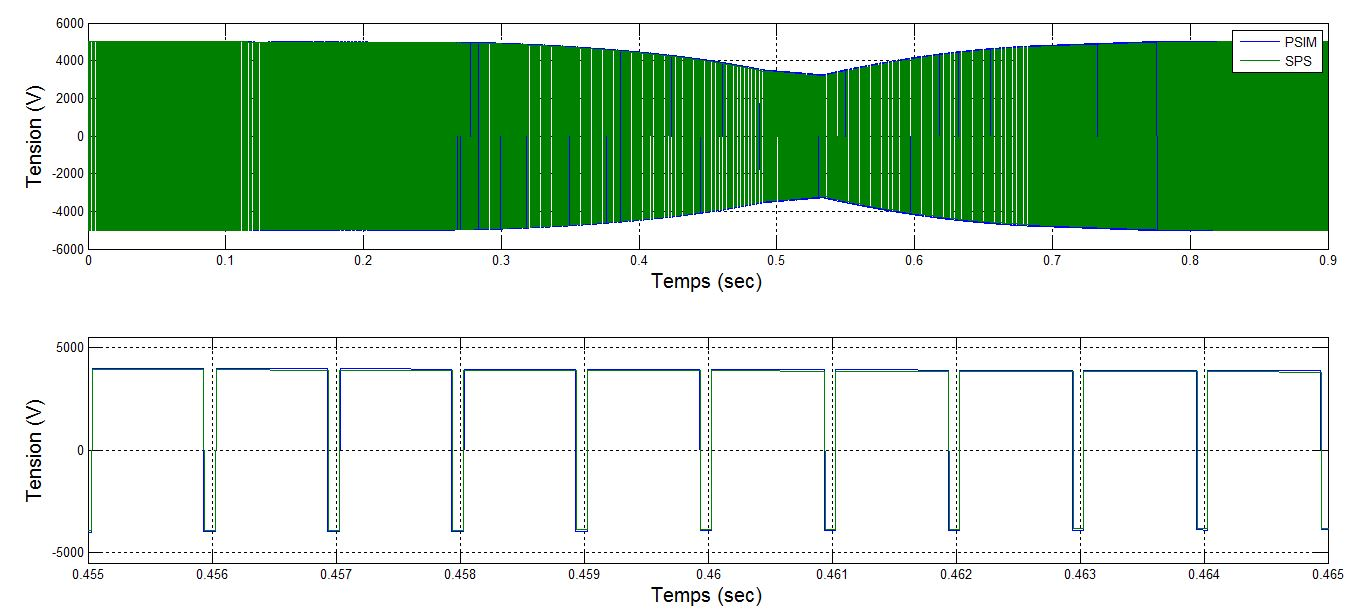
\includegraphics[scale=0.5]{Fig/Hach_AFE/1u/hach_ten_ch.jpg}
\caption{La tension au niveau de la charge à 1$\mu$s}
\label{AF_HA_CHV1}
\end{figure}

\begin{figure}[htb]
\centering
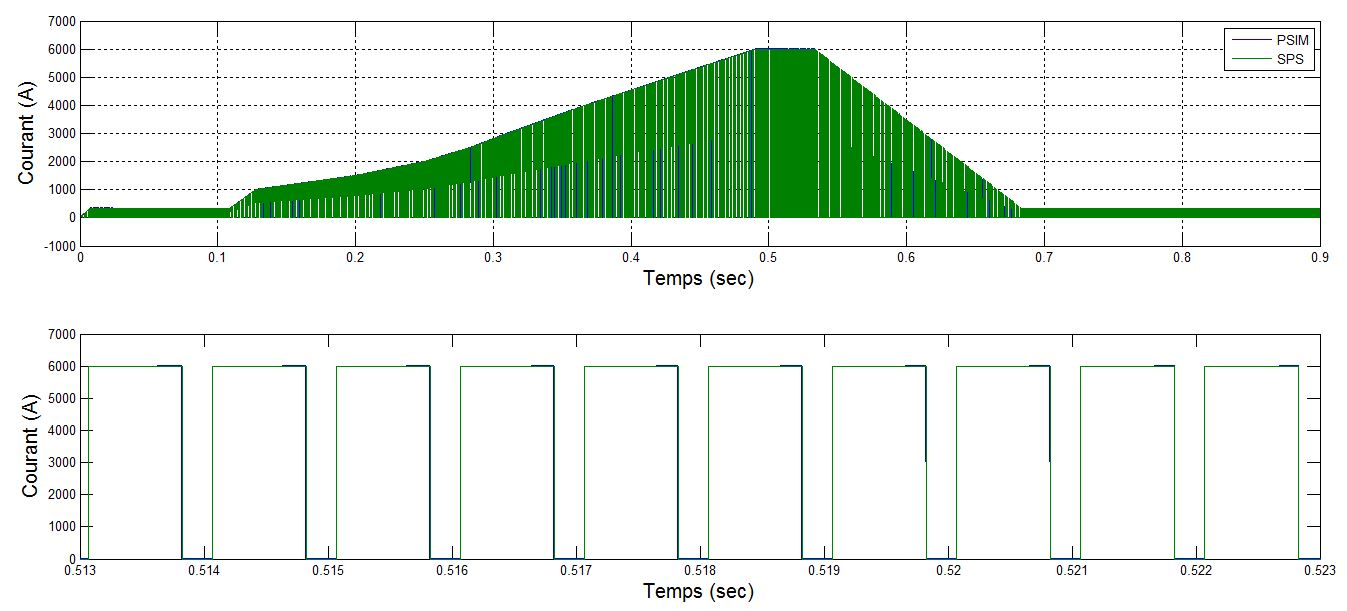
\includegraphics[scale=0.5]{Fig/Hach_AFE/1u/IGBT_cou_hach.jpg}
\caption{Le courant aux bornesu d'un IGBT à 1$\mu$s pour le hacheur 4 quadrants}
\label{AF_HA_HAA1}
\end{figure}

\begin{figure}[htb]
\centering
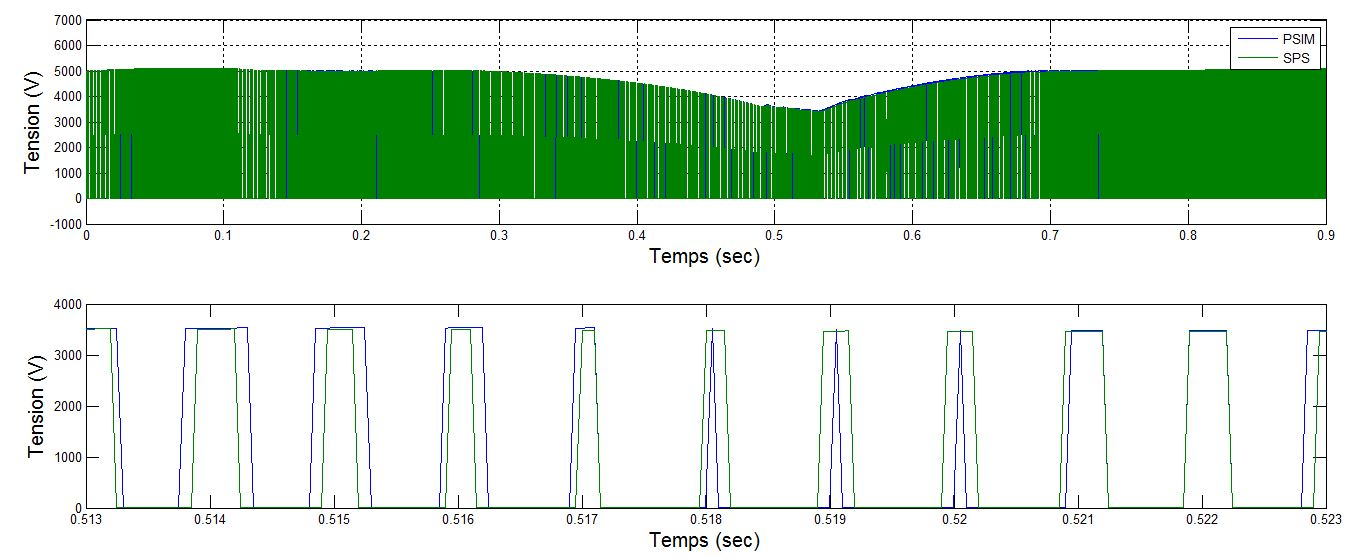
\includegraphics[scale=0.5]{Fig/Hach_AFE/1u/IGBT_ten_hach.jpg}
\caption{La tension aux bornes d'un IGBT à 1$\mu$s pour le hacheur 4 quadrants}
\label{AF_HA_HAV1}
\end{figure}



\clearpage
<<<<<<< HEAD
\section{AFE 3 niveaux NPC avec contrôle par MLI avec convertisseur CC-CC formé de 2 cellules NPC 3 niveaux}
Cette section présente les résultats de simulations obtenus sur PSIM et sur SPS pour le système complet, formé d'un redresseur AFE 3 niveaux avec régulation MLI et d'un convertisseur CC-CC composé de 2 cellules NPC 3 niveaux.  Le circuit électronique du système complet est présenté à la figure \ref{circuit_AFE_3L_RC_DCP_DCN}. Le tableau \ref{p_AF_DCP} présente les paramètres utilisés dans les sous-systèmes.

\begin{figure}[htb]
\centering
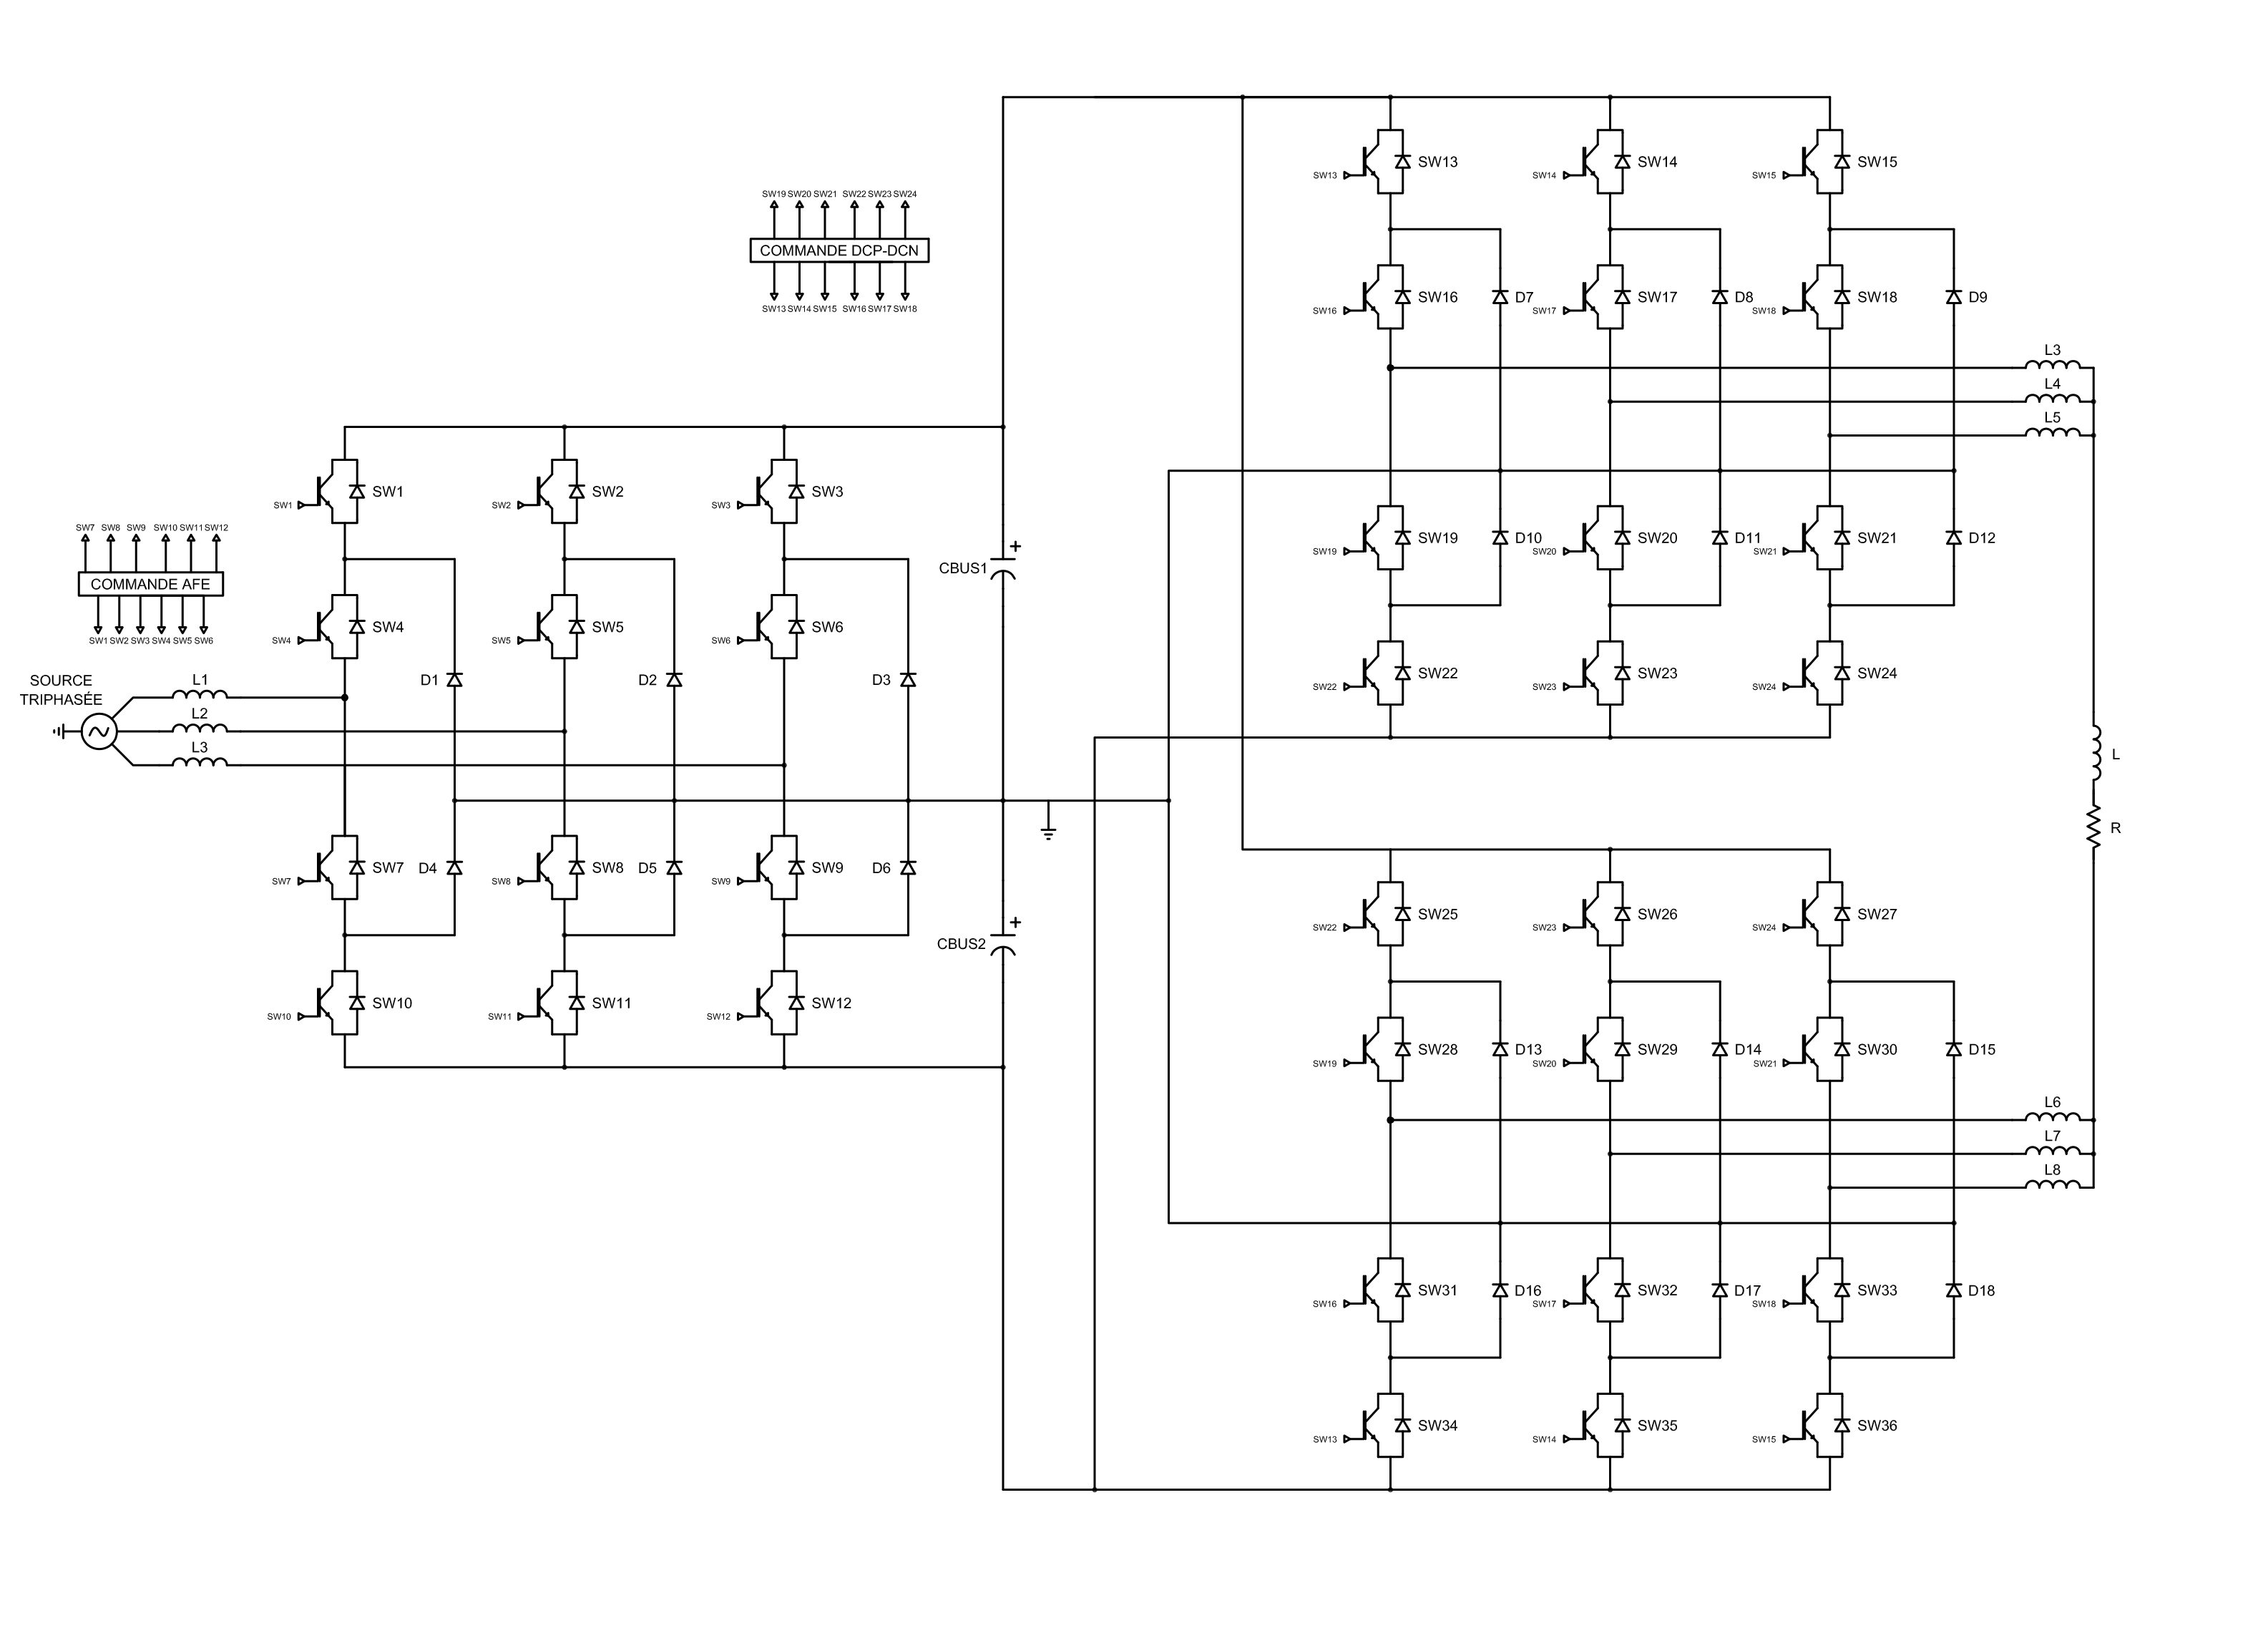
\includegraphics[scale=0.6]{Fig/AFE_3L_RC_DCP_DCN.png}
\caption{Circuit électrique de l'AFE 3 niveaux avec contrôle par hystérésis avec le DCP/DCN}
\label{circuit_AFE_3L_RC_DCP_DCN}
=======
\section{AFE 3 niveaux avec le DCP/DCN}
Cette section présente les résultats de simulations obtenus sur PSIM et sur SPS pour le système complet, formé d'un redresseur AFE 3 niveaux avec régulation MLI et d'un convertisseur CC-CC composé de 2 cellules NPC 3 niveaux.  La figure~\ref{AF3_DC} présente un schéma de l'implantation du système complet. Le tableau \ref{p_AF_DCP} présente les paramètres utilisés dans les sous-systèmes.

\begin{figure}[htb]
\centering
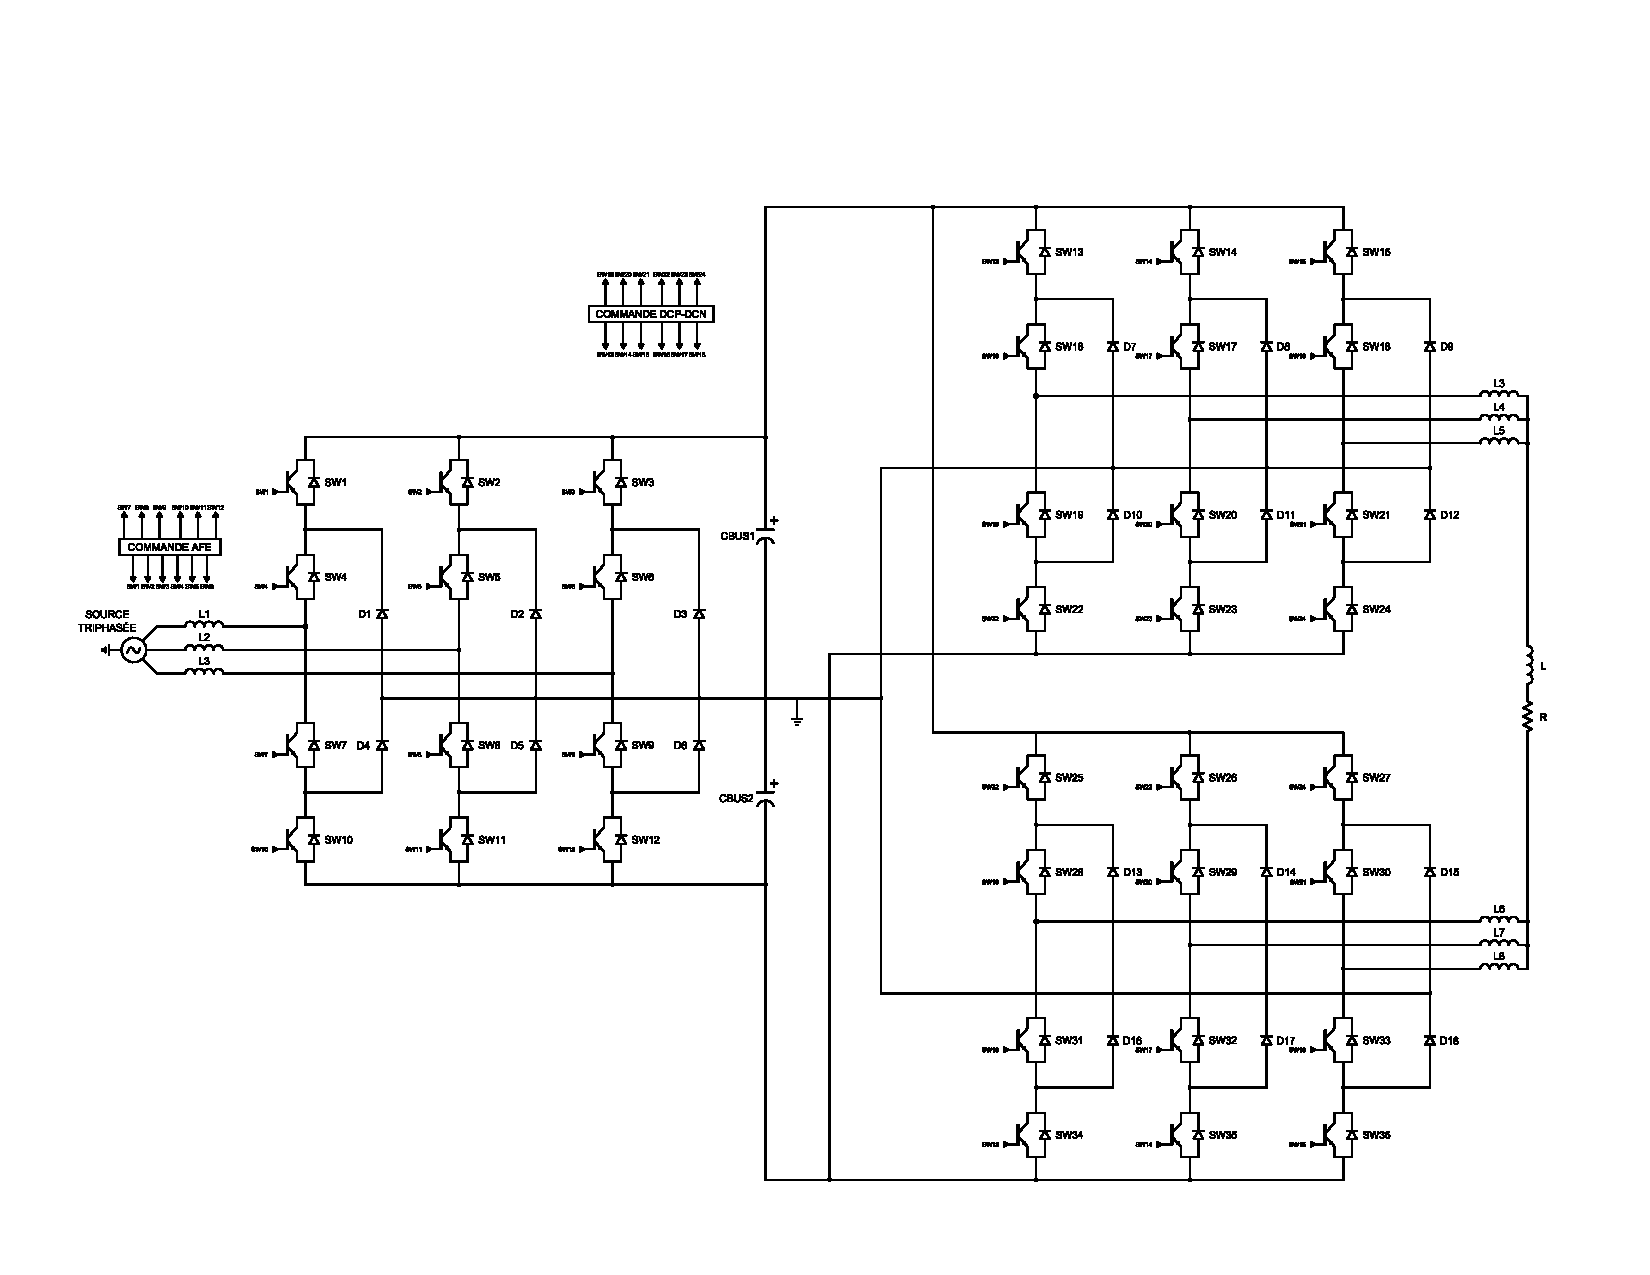
\includegraphics[scale=0.65]{Fig/DCP_AFE/AFE_3L_RC_DCP_DCN.pdf}
\caption{Circuit électrique de l'implémentation final de l'AFE 3 niveaux avec le DCP/DCN}
\label{AF3_DC}
>>>>>>> FETCH_HEAD
\end{figure}

\begin{table}[htb]
\centering
\begin{tabular}{|l|c|} 
  \hline
  \textbf{Paramètre} & \textbf{Valeur}  \\
  \hline\hline \hline
  \multicolumn{2}{|c|}{\textbf{AFE 3 niveaux}}\\ \hline \hline 
  Tension référence CC & 5000 V\\ \hline
  Fréquence de modulation & 1000 Hz \\ \hline
  Courant maximal à l'entrée& 1500A \\ \hline \hline
  \multicolumn{2}{|c|}{\textbf{IGBT AFE}}\\ \hline
  Résistance interne & 0.001 $\Omega$\\
  Résistance du snubber & 100k $\Omega$\\ \hline \hline
   \multicolumn{2}{|c|}{\textbf{PI courant AFE}}\\ \hline
  Gain proportionnel & 5 \\
  Gain intégrateur & 20 \\ \hline \hline
  \multicolumn{2}{|c|}{\textbf{PI commande AFE}}\\ \hline
  Rapport cyclique maximal & 0.95\\
  Gain proportionnel & 1.5611 \\
  Gain intégrateur & 24.6 \\ \hline \hline
  \multicolumn{2}{|c|}{\textbf{Bus CC}}\\ \hline
  Capacité & 330 mF\\
  \hline \hline \hline
  
  \multicolumn{2}{|c|}{\textbf{DCP/DCN}}\\ \hline \hline
  Fréquence de modulation & 333 Hz\\ \hline
  Rapport cyclique maximal & 1 \\ \hline
  Inductance de couplage & 10e-6 H \\ \hline \hline
  \multicolumn{2}{|c|}{\textbf{IGBT DCP/DCN}}\\ \hline
  Résistance interne & 0.001 $\Omega$\\
  Résistance du snubber & 100k $\Omega$\\ \hline \hline
   \multicolumn{2}{|c|}{\textbf{PI DCP/DCN}}\\ \hline
  Gain proportionnel & 1.5611 \\
  Gain intégrateur & 24.6 \\ \hline \hline
  \multicolumn{2}{|c|}{\textbf{Charge}}\\ \hline
  Résistance & 0.28 $\Omega$\\
  Inductance & 0.1 H \\
  \hline
\end{tabular}
\caption{Paramètres de simulation pour le DCP/DCN avec l'AFE 3 niveaux}
\label{p_AF_DCP}
\end{table}

\subsection{Vérification pour un pas de calcul de 1$\mu$s}
Cette section présente les résultats de simulations pour le système complet formé de l'AFE 3 niveaux avec régulation MLI et d'un convertisseur CC-CC composé de 2 cellules NPC 3 niveaux, pour un pas de calcul discret de 1$\mu$s. 

\begin{figure}[htb]
\centering
\includegraphics[scale=0.5]{Fig/DCP_AFE/1u/cour_al.jpg}
\caption{Le courant d'entrée de l'AFE pour un pas de calcul de 1$\mu$s}
\label{AF_DC_cou1}
\end{figure}


\begin{figure}[htb]
\centering
\includegraphics[scale=0.5]{Fig/DCP_AFE/1u/ten_bus.jpg}
\caption{La tension du bus CC pour un pas de calcul de 1$\mu$s}
\label{AF_DC_vch1}
\end{figure}



\begin{figure}[htb]
\centering
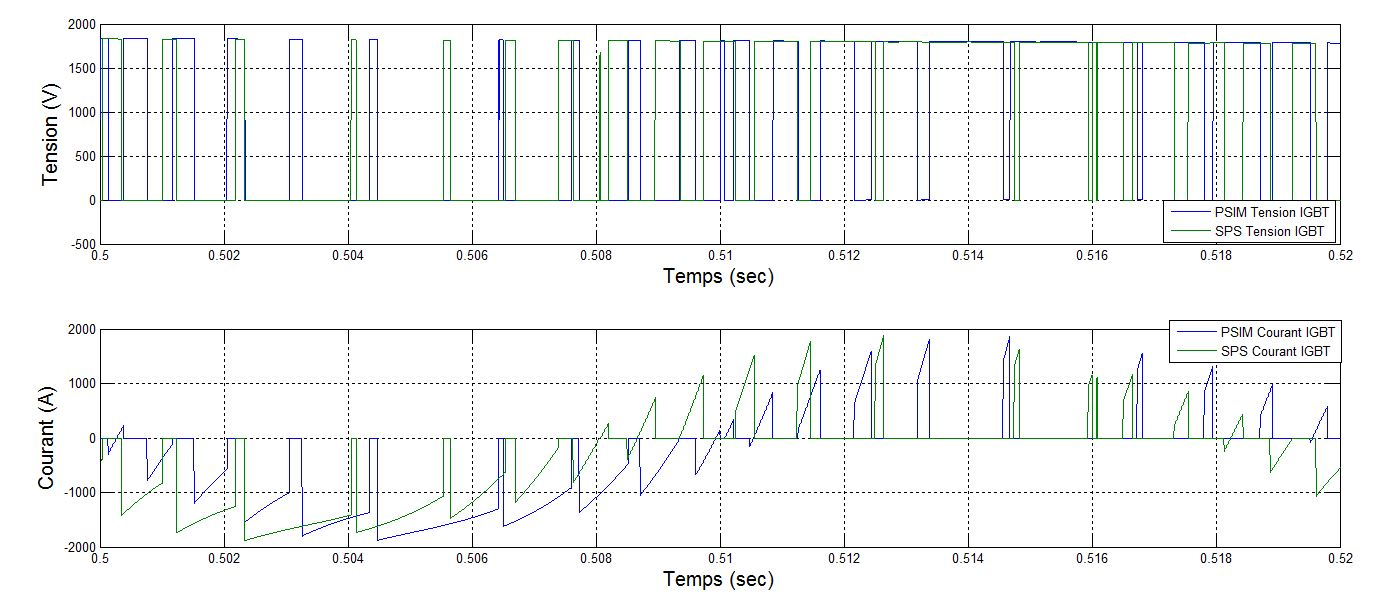
\includegraphics[scale=0.5]{Fig/DCP_AFE/1u/IGBT_afe.jpg}
\caption{La tension et le courant aux bornes d'un IGBT de l'AFE pour un pas de calcul de 1$\mu$s}
\label{AF_DC_IGBT1}
\end{figure}


\begin{figure}[htb]
\centering
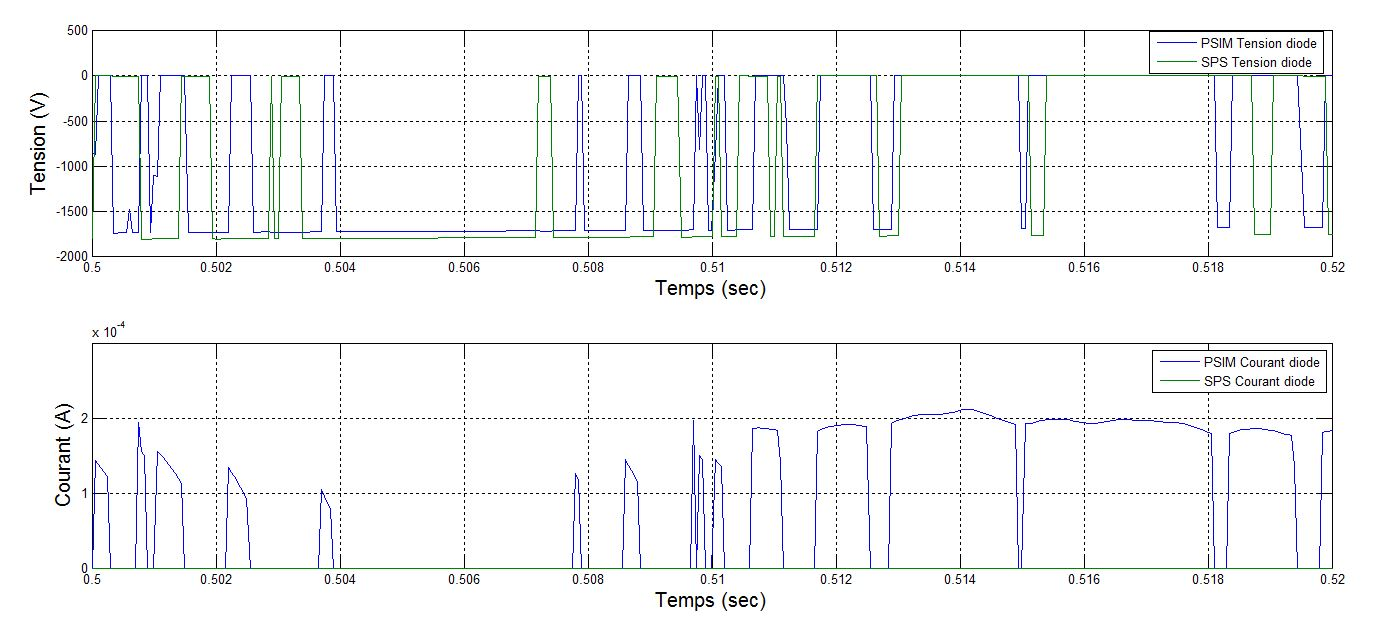
\includegraphics[scale=0.5]{Fig/DCP_AFE/1u/ten_diode_afe.jpg}
\caption{La tension et le courant aux bornes d'une diode de point milieu de l'AFE à 1$\mu$s}
\label{AF_DC_DI1}
\end{figure}


\begin{figure}[htb]
\centering
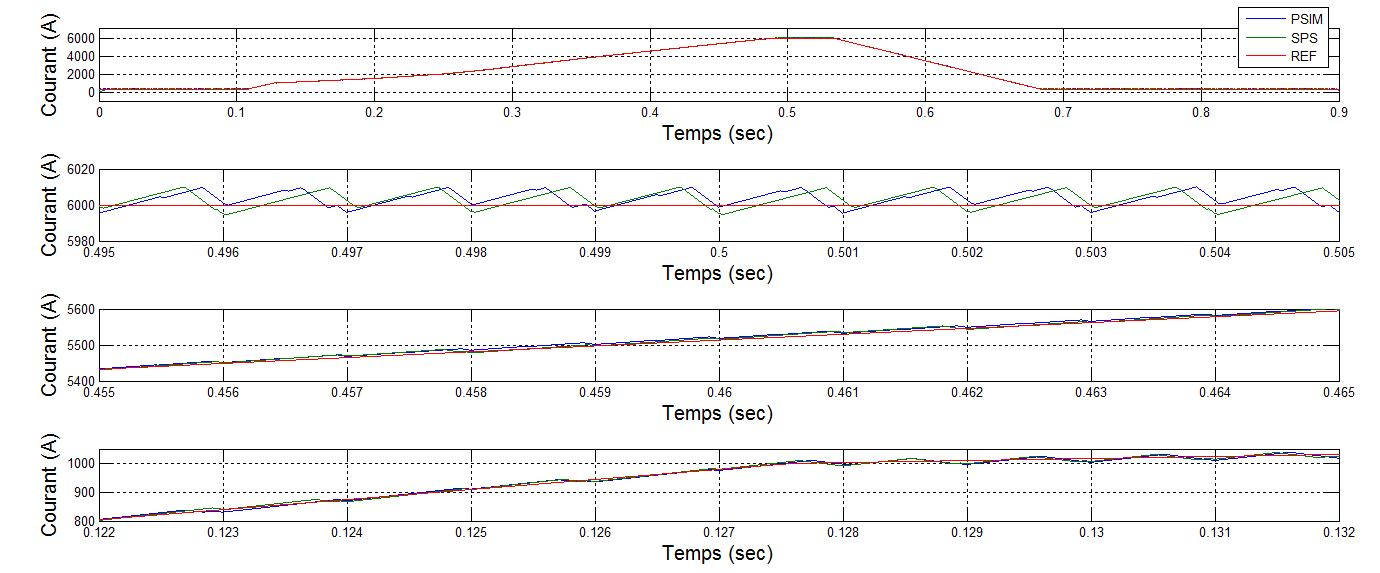
\includegraphics[scale=0.5]{Fig/DCP_AFE/1u/cour_ch.jpg}
\caption{Le courant aux bornes des électroaimants pour un pas de calcul de 1$\mu$s}
\label{AF_DC_CHA1}
\end{figure}



\begin{figure}[htb]
\centering
\includegraphics[scale=0.5]{Fig/DCP_AFE/1u/ten_ch.jpg}
\caption{La tension aux bornes des électroaimants pour un pas de calcul de 1$\mu$s}
\label{AF_DC_CHV1}
\end{figure}



\begin{figure}[htb]
\centering
\includegraphics[scale=0.5]{Fig/DCP_AFE/1u/hash_cou_IGBT.jpg}
\caption{Le courant traversant un IGBT du DCP/DCN pour un pas de calcul de à 1$\mu$s}
\label{AF_DC_HAA1}
\end{figure}



\begin{figure}[htb]
\centering
\includegraphics[scale=0.5]{Fig/DCP_AFE/1u/hash_ten_IGBT.jpg}
\caption{La tension aux bornes d'un IGBT du DCP/DCN pour un pas de calcul de 1$\mu$s}
\label{AF_DC_HAV1}
\end{figure}



\begin{figure}[htb]
\centering
\includegraphics[scale=0.5]{Fig/DCP_AFE/1u/hash_diode_cou.jpg}
\caption{Le courant traversant une diode de point milieu du DCP/DCN pour un pas de calcul d 1$\mu$s}
\label{AF_DC_HA1}
\end{figure}


\begin{figure}[htb]
\centering
\includegraphics[scale=0.5]{Fig/DCP_AFE/1u/hash_diode.jpg}
\caption{La tension aux bornes d'une diode de point milieu du DCP/DCN pour un pas de calcul de 1$\mu$s}
\label{AF_DC_HV1}
\end{figure}


\end{document}